\documentclass[journal]{IEEEtran}
\usepackage{cite}
\usepackage{amsmath,amssymb,amsfonts}
\usepackage{graphicx}
\usepackage{textcomp}
\usepackage{xcolor}
\usepackage{booktabs}
\usepackage{array}
\usepackage{multirow}
\usepackage{url}
\usepackage[hidelinks]{hyperref}
% AUTO-GENERATED by phishresearch.reporting - do not edit
\makeatletter
\newcommand{\res}[1]{\@ifundefined{r@#1}{\textbf{??#1??}}{\@nameuse{r@#1}}}
\@namedef{r@freezeHash}{069912e332d7}
\@namedef{r@nBoot}{2,000}
\@namedef{r@nAn}{73,575}
\@namedef{r@cAn}{46,769}
\@namedef{r@nAbenign}{36,400}
\@namedef{r@cAbenign}{22,167}
\@namedef{r@nAphishing}{37,175}
\@namedef{r@cAphishing}{24,602}
\@namedef{r@dupA}{18,811}
\@namedef{r@quarA}{3}
\@namedef{r@purgeA}{7,992}
\@namedef{r@lossBenignA}{25.9}
\@namedef{r@lossPhishA}{1.0}
\@namedef{r@groupsA}{20,913}
\@namedef{r@topGroupA}{wikipedia.org}
\@namedef{r@topGroupShareA}{2.9}
\@namedef{r@nBn}{92,500}
\@namedef{r@cBn}{75,077}
\@namedef{r@nBbenign}{46,250}
\@namedef{r@cBbenign}{29,758}
\@namedef{r@nBphishing}{46,250}
\@namedef{r@cBphishing}{45,319}
\@namedef{r@dupB}{1}
\@namedef{r@quarB}{17}
\@namedef{r@purgeB}{17,405}
\@namedef{r@lossBenignB}{35.6}
\@namedef{r@lossPhishB}{2.0}
\@namedef{r@groupsB}{6,735}
\@namedef{r@topGroupB}{za.com}
\@namedef{r@topGroupShareB}{11.0}
\@namedef{r@sharedGroups}{692}
\@namedef{r@exactOverlap}{33}
\@namedef{r@labelJoin}{73,575}
\@namedef{r@labelAgree}{100.0}
\@namedef{r@splitAFIT}{28,061}
\@namedef{r@splitGroupsAFIT}{8,018}
\@namedef{r@splitAVAL}{9,355}
\@namedef{r@splitGroupsAVAL}{6,448}
\@namedef{r@splitATEST}{9,353}
\@namedef{r@splitGroupsATEST}{6,447}
\@namedef{r@splitBFIT}{45,050}
\@namedef{r@splitGroupsBFIT}{2,614}
\@namedef{r@splitBVAL}{15,014}
\@namedef{r@splitGroupsBVAL}{2,060}
\@namedef{r@splitBTEST}{15,013}
\@namedef{r@splitGroupsBTEST}{2,061}
\@namedef{r@F1AARFALL}{0.895}
\@namedef{r@F1loAARFALL}{0.887}
\@namedef{r@F1hiAARFALL}{0.902}
\@namedef{r@APAARFALL}{0.962}
\@namedef{r@RecAARFALL}{0.475}
\@namedef{r@FPRAARFALL}{0.7}
\@namedef{r@F1dbAARFALL}{0.862}
\@namedef{r@F1AARFMEANPIbudget}{0.897}
\@namedef{r@F1loAARFMEANPIbudget}{0.889}
\@namedef{r@F1hiAARFMEANPIbudget}{0.904}
\@namedef{r@APAARFMEANPIbudget}{0.962}
\@namedef{r@RecAARFMEANPIbudget}{0.478}
\@namedef{r@FPRAARFMEANPIbudget}{0.8}
\@namedef{r@F1dbAARFMEANPIbudget}{0.865}
\@namedef{r@F1AARFSTABLEPIbudget}{0.896}
\@namedef{r@F1loAARFSTABLEPIbudget}{0.889}
\@namedef{r@F1hiAARFSTABLEPIbudget}{0.903}
\@namedef{r@APAARFSTABLEPIbudget}{0.962}
\@namedef{r@RecAARFSTABLEPIbudget}{0.468}
\@namedef{r@FPRAARFSTABLEPIbudget}{0.7}
\@namedef{r@F1dbAARFSTABLEPIbudget}{0.864}
\@namedef{r@F1AALGBMALL}{0.902}
\@namedef{r@F1loAALGBMALL}{0.894}
\@namedef{r@F1hiAALGBMALL}{0.909}
\@namedef{r@APAALGBMALL}{0.966}
\@namedef{r@RecAALGBMALL}{0.559}
\@namedef{r@FPRAALGBMALL}{0.9}
\@namedef{r@F1dbAALGBMALL}{0.872}
\@namedef{r@F1AALGBMMEANPIbudget}{0.900}
\@namedef{r@F1loAALGBMMEANPIbudget}{0.893}
\@namedef{r@F1hiAALGBMMEANPIbudget}{0.908}
\@namedef{r@APAALGBMMEANPIbudget}{0.965}
\@namedef{r@RecAALGBMMEANPIbudget}{0.553}
\@namedef{r@FPRAALGBMMEANPIbudget}{1.0}
\@namedef{r@F1dbAALGBMMEANPIbudget}{0.873}
\@namedef{r@F1AALGBMSTABLEPIbudget}{0.900}
\@namedef{r@F1loAALGBMSTABLEPIbudget}{0.892}
\@namedef{r@F1hiAALGBMSTABLEPIbudget}{0.907}
\@namedef{r@APAALGBMSTABLEPIbudget}{0.965}
\@namedef{r@RecAALGBMSTABLEPIbudget}{0.549}
\@namedef{r@FPRAALGBMSTABLEPIbudget}{1.0}
\@namedef{r@F1dbAALGBMSTABLEPIbudget}{0.873}
\@namedef{r@F1ABRFALL}{0.917}
\@namedef{r@F1loABRFALL}{0.905}
\@namedef{r@F1hiABRFALL}{0.929}
\@namedef{r@APABRFALL}{0.947}
\@namedef{r@RecABRFALL}{0.017}
\@namedef{r@FPRABRFALL}{0.3}
\@namedef{r@F1dbABRFALL}{0.782}
\@namedef{r@F1ABRFMEANPIbudget}{0.914}
\@namedef{r@F1loABRFMEANPIbudget}{0.901}
\@namedef{r@F1hiABRFMEANPIbudget}{0.925}
\@namedef{r@APABRFMEANPIbudget}{0.947}
\@namedef{r@RecABRFMEANPIbudget}{0.017}
\@namedef{r@FPRABRFMEANPIbudget}{0.3}
\@namedef{r@F1dbABRFMEANPIbudget}{0.767}
\@namedef{r@F1ABRFSTABLEPIbudget}{0.913}
\@namedef{r@F1loABRFSTABLEPIbudget}{0.901}
\@namedef{r@F1hiABRFSTABLEPIbudget}{0.924}
\@namedef{r@APABRFSTABLEPIbudget}{0.950}
\@namedef{r@RecABRFSTABLEPIbudget}{0.016}
\@namedef{r@FPRABRFSTABLEPIbudget}{0.2}
\@namedef{r@F1dbABRFSTABLEPIbudget}{0.763}
\@namedef{r@F1ABLGBMALL}{0.922}
\@namedef{r@F1loABLGBMALL}{0.910}
\@namedef{r@F1hiABLGBMALL}{0.933}
\@namedef{r@APABLGBMALL}{0.958}
\@namedef{r@RecABLGBMALL}{0.345}
\@namedef{r@FPRABLGBMALL}{1.6}
\@namedef{r@F1dbABLGBMALL}{0.796}
\@namedef{r@F1ABLGBMMEANPIbudget}{0.916}
\@namedef{r@F1loABLGBMMEANPIbudget}{0.903}
\@namedef{r@F1hiABLGBMMEANPIbudget}{0.927}
\@namedef{r@APABLGBMMEANPIbudget}{0.956}
\@namedef{r@RecABLGBMMEANPIbudget}{0.510}
\@namedef{r@FPRABLGBMMEANPIbudget}{1.8}
\@namedef{r@F1dbABLGBMMEANPIbudget}{0.778}
\@namedef{r@F1ABLGBMSTABLEPIbudget}{0.915}
\@namedef{r@F1loABLGBMSTABLEPIbudget}{0.902}
\@namedef{r@F1hiABLGBMSTABLEPIbudget}{0.927}
\@namedef{r@APABLGBMSTABLEPIbudget}{0.956}
\@namedef{r@RecABLGBMSTABLEPIbudget}{0.482}
\@namedef{r@FPRABLGBMSTABLEPIbudget}{1.7}
\@namedef{r@F1dbABLGBMSTABLEPIbudget}{0.776}
\@namedef{r@F1BBRFALL}{0.956}
\@namedef{r@F1loBBRFALL}{0.947}
\@namedef{r@F1hiBBRFALL}{0.964}
\@namedef{r@APBBRFALL}{0.993}
\@namedef{r@RecBBRFALL}{0.831}
\@namedef{r@FPRBBRFALL}{0.4}
\@namedef{r@F1dbBBRFALL}{0.916}
\@namedef{r@F1BBRFMEANPIbudget}{0.941}
\@namedef{r@F1loBBRFMEANPIbudget}{0.930}
\@namedef{r@F1hiBBRFMEANPIbudget}{0.950}
\@namedef{r@APBBRFMEANPIbudget}{0.989}
\@namedef{r@RecBBRFMEANPIbudget}{0.823}
\@namedef{r@FPRBBRFMEANPIbudget}{0.6}
\@namedef{r@F1dbBBRFMEANPIbudget}{0.888}
\@namedef{r@F1BBRFSTABLEPIbudget}{0.944}
\@namedef{r@F1loBBRFSTABLEPIbudget}{0.933}
\@namedef{r@F1hiBBRFSTABLEPIbudget}{0.953}
\@namedef{r@APBBRFSTABLEPIbudget}{0.989}
\@namedef{r@RecBBRFSTABLEPIbudget}{0.820}
\@namedef{r@FPRBBRFSTABLEPIbudget}{0.8}
\@namedef{r@F1dbBBRFSTABLEPIbudget}{0.904}
\@namedef{r@F1BBLGBMALL}{0.958}
\@namedef{r@F1loBBLGBMALL}{0.949}
\@namedef{r@F1hiBBLGBMALL}{0.966}
\@namedef{r@APBBLGBMALL}{0.993}
\@namedef{r@RecBBLGBMALL}{0.876}
\@namedef{r@FPRBBLGBMALL}{0.5}
\@namedef{r@F1dbBBLGBMALL}{0.936}
\@namedef{r@F1BBLGBMMEANPIbudget}{0.942}
\@namedef{r@F1loBBLGBMMEANPIbudget}{0.932}
\@namedef{r@F1hiBBLGBMMEANPIbudget}{0.951}
\@namedef{r@APBBLGBMMEANPIbudget}{0.990}
\@namedef{r@RecBBLGBMMEANPIbudget}{0.820}
\@namedef{r@FPRBBLGBMMEANPIbudget}{0.2}
\@namedef{r@F1dbBBLGBMMEANPIbudget}{0.871}
\@namedef{r@F1BBLGBMSTABLEPIbudget}{0.946}
\@namedef{r@F1loBBLGBMSTABLEPIbudget}{0.937}
\@namedef{r@F1hiBBLGBMSTABLEPIbudget}{0.955}
\@namedef{r@APBBLGBMSTABLEPIbudget}{0.990}
\@namedef{r@RecBBLGBMSTABLEPIbudget}{0.821}
\@namedef{r@FPRBBLGBMSTABLEPIbudget}{0.3}
\@namedef{r@F1dbBBLGBMSTABLEPIbudget}{0.895}
\@namedef{r@F1BARFALL}{0.739}
\@namedef{r@F1loBARFALL}{0.727}
\@namedef{r@F1hiBARFALL}{0.751}
\@namedef{r@APBARFALL}{0.829}
\@namedef{r@RecBARFALL}{0.115}
\@namedef{r@FPRBARFALL}{1.4}
\@namedef{r@F1dbBARFALL}{0.703}
\@namedef{r@F1BARFMEANPIbudget}{0.639}
\@namedef{r@F1loBARFMEANPIbudget}{0.625}
\@namedef{r@F1hiBARFMEANPIbudget}{0.652}
\@namedef{r@APBARFMEANPIbudget}{0.739}
\@namedef{r@RecBARFMEANPIbudget}{0.101}
\@namedef{r@FPRBARFMEANPIbudget}{2.2}
\@namedef{r@F1dbBARFMEANPIbudget}{0.604}
\@namedef{r@F1BARFSTABLEPIbudget}{0.697}
\@namedef{r@F1loBARFSTABLEPIbudget}{0.685}
\@namedef{r@F1hiBARFSTABLEPIbudget}{0.710}
\@namedef{r@APBARFSTABLEPIbudget}{0.746}
\@namedef{r@RecBARFSTABLEPIbudget}{0.135}
\@namedef{r@FPRBARFSTABLEPIbudget}{3.1}
\@namedef{r@F1dbBARFSTABLEPIbudget}{0.649}
\@namedef{r@F1BALGBMALL}{0.790}
\@namedef{r@F1loBALGBMALL}{0.779}
\@namedef{r@F1hiBALGBMALL}{0.800}
\@namedef{r@APBALGBMALL}{0.883}
\@namedef{r@RecBALGBMALL}{0.440}
\@namedef{r@FPRBALGBMALL}{3.2}
\@namedef{r@F1dbBALGBMALL}{0.747}
\@namedef{r@F1BALGBMMEANPIbudget}{0.619}
\@namedef{r@F1loBALGBMMEANPIbudget}{0.605}
\@namedef{r@F1hiBALGBMMEANPIbudget}{0.634}
\@namedef{r@APBALGBMMEANPIbudget}{0.772}
\@namedef{r@RecBALGBMMEANPIbudget}{0.143}
\@namedef{r@FPRBALGBMMEANPIbudget}{0.9}
\@namedef{r@F1dbBALGBMMEANPIbudget}{0.588}
\@namedef{r@F1BALGBMSTABLEPIbudget}{0.697}
\@namedef{r@F1loBALGBMSTABLEPIbudget}{0.685}
\@namedef{r@F1hiBALGBMSTABLEPIbudget}{0.709}
\@namedef{r@APBALGBMSTABLEPIbudget}{0.790}
\@namedef{r@RecBALGBMSTABLEPIbudget}{0.220}
\@namedef{r@FPRBALGBMSTABLEPIbudget}{2.2}
\@namedef{r@F1dbBALGBMSTABLEPIbudget}{0.653}
\@namedef{r@DropALGBMALL}{-2.0}
\@namedef{r@DropALGBMMEANPIbudget}{-1.5}
\@namedef{r@DropALGBMMEANPImatched}{-1.5}
\@namedef{r@DropALGBMSTABLEPIbudget}{-1.6}
\@namedef{r@DropALGBMSTABLEPImatched}{-1.6}
\@namedef{r@DropARFALL}{-2.3}
\@namedef{r@DropARFMEANPIbudget}{-1.7}
\@namedef{r@DropARFMEANPImatched}{-1.7}
\@namedef{r@DropARFSTABLEPIbudget}{-1.7}
\@namedef{r@DropARFSTABLEPImatched}{-1.7}
\@namedef{r@DropBLGBMALL}{16.9}
\@namedef{r@DropBLGBMMEANPIbudget}{32.3}
\@namedef{r@DropBLGBMMEANPImatched}{32.3}
\@namedef{r@DropBLGBMSTABLEPIbudget}{25.0}
\@namedef{r@DropBLGBMSTABLEPImatched}{25.0}
\@namedef{r@DropBRFALL}{21.7}
\@namedef{r@DropBRFMEANPIbudget}{30.2}
\@namedef{r@DropBRFMEANPImatched}{30.2}
\@namedef{r@DropBRFSTABLEPIbudget}{24.7}
\@namedef{r@DropBRFSTABLEPImatched}{24.7}
\@namedef{r@DropMin}{-2.3}
\@namedef{r@DropMax}{21.7}
\@namedef{r@DeltaABRF}{-0.000}
\@namedef{r@DeltaLoABRF}{-0.001}
\@namedef{r@DeltaHiABRF}{+0.000}
\@namedef{r@DeltaABLGBM}{-0.000}
\@namedef{r@DeltaLoABLGBM}{-0.001}
\@namedef{r@DeltaHiABLGBM}{+0.000}
\@namedef{r@DeltaBARF}{+0.059}
\@namedef{r@DeltaLoBARF}{+0.051}
\@namedef{r@DeltaHiBARF}{+0.066}
\@namedef{r@DeltaBALGBM}{+0.077}
\@namedef{r@DeltaLoBALGBM}{+0.069}
\@namedef{r@DeltaHiBALGBM}{+0.086}
\@namedef{r@nPrimaryExcl}{2}
\@namedef{r@nPrimaryPos}{2}
\@namedef{r@nPrimaryEff}{2}
\@namedef{r@SecABRFSTABLEALL}{-0.004}
\@namedef{r@SecABRFMEANALL}{-0.004}
\@namedef{r@SecABRFSTABLE}{-0.000}
\@namedef{r@SecABLGBMSTABLEALL}{-0.007}
\@namedef{r@SecABLGBMMEANALL}{-0.006}
\@namedef{r@SecABLGBMSTABLE}{-0.000}
\@namedef{r@SecBARFSTABLEALL}{-0.042}
\@namedef{r@SecBARFMEANALL}{-0.100}
\@namedef{r@SecBARFSTABLE}{+0.059}
\@namedef{r@SecBALGBMSTABLEALL}{-0.093}
\@namedef{r@SecBALGBMMEANALL}{-0.170}
\@namedef{r@SecBALGBMSTABLE}{+0.077}
\@namedef{r@highCorrA}{14}
\@namedef{r@piSecA}{26.1}
\@namedef{r@highCorrB}{17}
\@namedef{r@piSecB}{10.6}
\@namedef{r@relLatB1Min}{0.75}
\@namedef{r@relLatB1Max}{1.10}
\@namedef{r@relLatBkMin}{0.47}
\@namedef{r@relLatBkMax}{1.01}
\@namedef{r@extractShareMedian}{10.4}
\@namedef{r@cpu}{Intel64 Family 6 Model 154 Stepping 3, GenuineIntel}
\@namedef{r@ram}{32}
\@namedef{r@pyver}{3.10.0}
\@namedef{r@RhoALGBMALL}{0.99}
\@namedef{r@RhoALGBMSTABLEPIbudget}{0.88}
\@namedef{r@RhoARFALL}{0.97}
\@namedef{r@RhoARFSTABLEPIbudget}{0.81}
\@namedef{r@RhoBLGBMALL}{0.96}
\@namedef{r@RhoBLGBMSTABLEPIbudget}{0.98}
\@namedef{r@RhoBRFALL}{0.95}
\@namedef{r@RhoBRFSTABLEPIbudget}{0.98}
\@namedef{r@shapAddErr}{2.9e-08}
\@namedef{r@rhoMin}{0.81}
\@namedef{r@rhoMax}{0.99}
\@namedef{r@rhoSeedMin}{1.00}
\@namedef{r@medLenABenign}{55}
\@namedef{r@medDotsABenign}{2}
\@namedef{r@medSubABenign}{1}
\@namedef{r@httpsABenign}{34.9}
\@namedef{r@medLenAPhish}{63}
\@namedef{r@medDotsAPhish}{2}
\@namedef{r@medSubAPhish}{0}
\@namedef{r@httpsAPhish}{1.5}
\@namedef{r@medLenBBenign}{41}
\@namedef{r@medDotsBBenign}{2}
\@namedef{r@medSubBBenign}{1}
\@namedef{r@httpsBBenign}{83.5}
\@namedef{r@medLenBPhish}{74}
\@namedef{r@medDotsBPhish}{5}
\@namedef{r@medSubBPhish}{3}
\@namedef{r@httpsBPhish}{30.6}
\@namedef{r@status}{benchmark: completed, evaluation: completed, shap: completed}
\makeatother

% AUTO-GENERATED by phishresearch.extensions.report from extensions/run_20261116T063740629948Z_fe541b37 - do not edit
\makeatletter
\@namedef{r@xRuleSrcA}{0.739}
\@namedef{r@xRuleTgtA}{0.874}
\@namedef{r@xRuleTgtAPA}{0.858}
\@namedef{r@xRuleTgtAUCA}{0.855}
\@namedef{r@xRuleTgtRecA}{0.845}
\@namedef{r@xRuleTgtFPRA}{13.5}
\@namedef{r@xLRSrcA}{0.871}
\@namedef{r@xLRTgtA}{0.275}
\@namedef{r@xLRTgtAPA}{0.840}
\@namedef{r@xLRTgtAUCA}{0.847}
\@namedef{r@xLRTgtRecA}{0.168}
\@namedef{r@xLRTgtFPRA}{8.6}
\@namedef{r@xRFSrcA}{0.903}
\@namedef{r@xRFTgtA}{0.918}
\@namedef{r@xRFTgtAPA}{0.966}
\@namedef{r@xRFTgtAUCA}{0.961}
\@namedef{r@xRFTgtRecA}{0.891}
\@namedef{r@xRFTgtFPRA}{7.7}
\@namedef{r@xLGBMSrcA}{0.909}
\@namedef{r@xLGBMTgtA}{0.928}
\@namedef{r@xLGBMTgtAPA}{0.972}
\@namedef{r@xLGBMTgtAUCA}{0.968}
\@namedef{r@xLGBMTgtRecA}{0.898}
\@namedef{r@xLGBMTgtFPRA}{5.7}
\@namedef{r@xRFnoHSrcA}{0.897}
\@namedef{r@xRFnoHTgtA}{0.898}
\@namedef{r@xRFnoHTgtAPA}{0.921}
\@namedef{r@xRFnoHTgtAUCA}{0.933}
\@namedef{r@xRFnoHTgtRecA}{0.958}
\@namedef{r@xRFnoHTgtFPRA}{26.7}
\@namedef{r@xLGBMnoHSrcA}{0.899}
\@namedef{r@xLGBMnoHTgtA}{0.906}
\@namedef{r@xLGBMnoHTgtAPA}{0.946}
\@namedef{r@xLGBMnoHTgtAUCA}{0.942}
\@namedef{r@xLGBMnoHTgtRecA}{0.947}
\@namedef{r@xLGBMnoHTgtFPRA}{21.9}
\@namedef{r@xRuleSrcB}{0.874}
\@namedef{r@xRuleTgtB}{0.739}
\@namedef{r@xRuleTgtAPB}{0.593}
\@namedef{r@xRuleTgtAUCB}{0.618}
\@namedef{r@xRuleTgtRecB}{0.976}
\@namedef{r@xRuleTgtFPRB}{74.0}
\@namedef{r@xLRSrcB}{0.929}
\@namedef{r@xLRTgtB}{0.666}
\@namedef{r@xLRTgtAPB}{0.749}
\@namedef{r@xLRTgtAUCB}{0.763}
\@namedef{r@xLRTgtRecB}{0.589}
\@namedef{r@xLRTgtFPRB}{19.9}
\@namedef{r@xRFSrcB}{0.951}
\@namedef{r@xRFTgtB}{0.734}
\@namedef{r@xRFTgtAPB}{0.826}
\@namedef{r@xRFTgtAUCB}{0.821}
\@namedef{r@xRFTgtRecB}{0.672}
\@namedef{r@xRFTgtFPRB}{17.6}
\@namedef{r@xLGBMSrcB}{0.955}
\@namedef{r@xLGBMTgtB}{0.783}
\@namedef{r@xLGBMTgtAPB}{0.874}
\@namedef{r@xLGBMTgtAUCB}{0.863}
\@namedef{r@xLGBMTgtRecB}{0.772}
\@namedef{r@xLGBMTgtFPRB}{22.1}
\@namedef{r@xRFnoHSrcB}{0.951}
\@namedef{r@xRFnoHTgtB}{0.692}
\@namedef{r@xRFnoHTgtAPB}{0.812}
\@namedef{r@xRFnoHTgtAUCB}{0.792}
\@namedef{r@xRFnoHTgtRecB}{0.598}
\@namedef{r@xRFnoHTgtFPRB}{14.6}
\@namedef{r@xLGBMnoHSrcB}{0.956}
\@namedef{r@xLGBMnoHTgtB}{0.716}
\@namedef{r@xLGBMnoHTgtAPB}{0.852}
\@namedef{r@xLGBMnoHTgtAUCB}{0.834}
\@namedef{r@xLGBMnoHTgtRecB}{0.638}
\@namedef{r@xLGBMnoHTgtFPRB}{16.0}
\@namedef{r@xDsRFLRA}{+0.032}
\@namedef{r@xDsRFLRACI}{[+0.026, +0.038]}
\@namedef{r@xDRFLRA}{+0.643}
\@namedef{r@xDRFLRACI}{[+0.611, +0.674]}
\@namedef{r@xDsLGBMLRA}{+0.037}
\@namedef{r@xDsLGBMLRACI}{[+0.031, +0.044]}
\@namedef{r@xDLGBMLRA}{+0.653}
\@namedef{r@xDLGBMLRACI}{[+0.622, +0.682]}
\@namedef{r@xDsRFnoHA}{+0.007}
\@namedef{r@xDsRFnoHACI}{[+0.003, +0.010]}
\@namedef{r@xDRFnoHA}{+0.020}
\@namedef{r@xDRFnoHACI}{[+0.007, +0.032]}
\@namedef{r@xDsLGBMnoHA}{+0.010}
\@namedef{r@xDsLGBMnoHACI}{[+0.006, +0.014]}
\@namedef{r@xDLGBMnoHA}{+0.022}
\@namedef{r@xDLGBMnoHACI}{[+0.010, +0.034]}
\@namedef{r@xDsRFLRB}{+0.022}
\@namedef{r@xDsRFLRBCI}{[+0.014, +0.030]}
\@namedef{r@xDRFLRB}{+0.068}
\@namedef{r@xDRFLRBCI}{[+0.055, +0.080]}
\@namedef{r@xDsLGBMLRB}{+0.027}
\@namedef{r@xDsLGBMLRBCI}{[+0.018, +0.034]}
\@namedef{r@xDLGBMLRB}{+0.117}
\@namedef{r@xDLGBMLRBCI}{[+0.104, +0.131]}
\@namedef{r@xDsRFnoHB}{-0.000}
\@namedef{r@xDsRFnoHBCI}{[-0.002, +0.001]}
\@namedef{r@xDRFnoHB}{+0.042}
\@namedef{r@xDRFnoHBCI}{[+0.037, +0.048]}
\@namedef{r@xDsLGBMnoHB}{-0.001}
\@namedef{r@xDsLGBMnoHBCI}{[-0.003, +0.001]}
\@namedef{r@xDLGBMnoHB}{+0.067}
\@namedef{r@xDLGBMnoHBCI}{[+0.060, +0.075]}
\@namedef{r@xAHttpsHTTPSFPR}{1.9}
\@namedef{r@xAHttpsHTTPSFNR}{57.4}
\@namedef{r@xAHttpsHTTPSShare}{44}
\@namedef{r@xAHttpsnotHTTPSFPR}{30.2}
\@namedef{r@xAHttpsnotHTTPSFNR}{1.6}
\@namedef{r@xAHttpsnotHTTPSShare}{56}
\@namedef{r@xASub0FPR}{7.5}
\@namedef{r@xASub0FNR}{35.5}
\@namedef{r@xASub0Share}{19}
\@namedef{r@xASub1FPR}{4.0}
\@namedef{r@xASub1FNR}{49.4}
\@namedef{r@xASub1Share}{33}
\@namedef{r@xASubge2FPR}{22.6}
\@namedef{r@xASubge2FNR}{0.6}
\@namedef{r@xASubge2Share}{48}
\@namedef{r@xBHttpsHTTPSFPR}{11.7}
\@namedef{r@xBHttpsHTTPSFNR}{33.3}
\@namedef{r@xBHttpsHTTPSShare}{14}
\@namedef{r@xBHttpsnotHTTPSFPR}{25.7}
\@namedef{r@xBHttpsnotHTTPSFNR}{22.5}
\@namedef{r@xBHttpsnotHTTPSShare}{86}
\@namedef{r@xBSub0FPR}{51.9}
\@namedef{r@xBSub0FNR}{10.5}
\@namedef{r@xBSub0Share}{49}
\@namedef{r@xBSub1FPR}{10.9}
\@namedef{r@xBSub1FNR}{53.2}
\@namedef{r@xBSub1Share}{49}
\@namedef{r@xBSubge2FPR}{18.8}
\@namedef{r@xBSubge2FNR}{13.4}
\@namedef{r@xBSubge2Share}{2}
\@namedef{r@xdF01A}{+0.44}
\@namedef{r@xdF01B}{+0.72}
\@namedef{r@xdF02A}{+0.12}
\@namedef{r@xdF02B}{+2.11}
\@namedef{r@xdF03A}{+0.04}
\@namedef{r@xdF03B}{+0.09}
\@namedef{r@xdF06A}{+0.39}
\@namedef{r@xdF06B}{+1.75}
\@namedef{r@xdF07A}{-0.61}
\@namedef{r@xdF07B}{-0.17}
\@namedef{r@xdF16A}{+0.55}
\@namedef{r@xdF16B}{+0.16}
\@namedef{r@xdF18A}{+0.54}
\@namedef{r@xdF18B}{+0.03}
\@namedef{r@xdF20A}{+0.42}
\@namedef{r@xdF20B}{+1.04}
\@namedef{r@xdF22A}{-0.38}
\@namedef{r@xdF22B}{+1.43}
\@namedef{r@xdF23A}{-0.58}
\@namedef{r@xdF23B}{+1.54}
\@namedef{r@xdF29A}{+0.74}
\@namedef{r@xdF29B}{-0.34}
\@namedef{r@xdF30A}{-0.98}
\@namedef{r@xdF30B}{-1.23}
\@namedef{r@xdF35A}{+0.77}
\@namedef{r@xdF35B}{+0.29}
\@namedef{r@xdF36A}{+0.51}
\@namedef{r@xdF36B}{+0.18}
\@namedef{r@xFlipList}{\texttt{host\_label\_count}, \texttt{subdomain\_label\_count}, \texttt{has\_query}}
\@namedef{r@xNFlip}{3}
\@namedef{r@xNEda}{14}
\@namedef{r@xHttpsBenignA}{34.9}
\@namedef{r@xHttpsPhishA}{1.5}
\@namedef{r@xHttpsBenignB}{83.5}
\@namedef{r@xHttpsPhishB}{30.6}
\makeatother

% AUTO-GENERATED by phishresearch.extensions.report (DA-GAFS) from extensions/dagafs/run_20261116T114100735204Z_67293905 - do not edit
\makeatletter
\@namedef{r@gK}{35}
\@namedef{r@gKI}{12}
\@namedef{r@gKIS}{13}
\@namedef{r@gKISD}{35}
\@namedef{r@gNConflict}{2}
\@namedef{r@gConflictList}{\texttt{host\_label\_count}, \texttt{subdomain\_label\_count}}
\@namedef{r@gFeatList}{\texttt{url\_length}, \texttt{host\_length}, \texttt{path\_length}, \texttt{query\_length}, \texttt{fragment\_length}, \texttt{dot\_count}, \texttt{hyphen\_count}, \texttt{underscore\_count}, \texttt{slash\_count}, \texttt{at\_count}, \texttt{question\_count}, \texttt{equals\_count}, \texttt{ampersand\_count}, \texttt{percent\_count}, \texttt{colon\_count}, \texttt{digit\_count}, \texttt{letter\_count}, \texttt{digit\_ratio}, \texttt{nonascii\_count}, \texttt{char\_entropy}, \texttt{max\_alnum\_run}, \texttt{subdomain\_label\_count}, \texttt{host\_digit\_ratio}, \texttt{host\_is\_ip}, \texttt{explicit\_port}, \texttt{has\_userinfo}, \texttt{has\_query}, \texttt{is\_https}, \texttt{scheme\_missing}, \texttt{host\_has\_punycode}, \texttt{encoded\_triplet\_count}, \texttt{query\_pair\_count}, \texttt{path\_segment\_count}, \texttt{url\_keyword\_count}, \texttt{host\_keyword\_count}}
\@namedef{r@gNfeat}{37}
\@namedef{r@gSignStabMin}{1.00}
\@namedef{r@grF01A}{+0.20}
\@namedef{r@grF01B}{+0.69}
\@namedef{r@gSF01}{0.33}
\@namedef{r@gIF01}{0.03}
\@namedef{r@grF02A}{+0.02}
\@namedef{r@grF02B}{+0.87}
\@namedef{r@gSF02}{0.61}
\@namedef{r@gIF02}{0.53}
\@namedef{r@grF03A}{-0.01}
\@namedef{r@grF03B}{+0.29}
\@namedef{r@gSF03}{1.00}
\@namedef{r@gIF03}{0.08}
\@namedef{r@grF04A}{+0.26}
\@namedef{r@grF04B}{-0.09}
\@namedef{r@gSF04}{0.33}
\@namedef{r@gIF04}{0.04}
\@namedef{r@grF05A}{+0.01}
\@namedef{r@grF05B}{+0.00}
\@namedef{r@gSF05}{0.00}
\@namedef{r@gIF05}{0.00}
\@namedef{r@grF06A}{+0.12}
\@namedef{r@grF06B}{+0.77}
\@namedef{r@gSF06}{1.00}
\@namedef{r@gIF06}{0.17}
\@namedef{r@grF07A}{-0.23}
\@namedef{r@grF07B}{-0.11}
\@namedef{r@gSF07}{0.50}
\@namedef{r@gIF07}{0.11}
\@namedef{r@grF08A}{-0.11}
\@namedef{r@grF08B}{-0.08}
\@namedef{r@gSF08}{0.11}
\@namedef{r@gIF08}{0.03}
\@namedef{r@grF09A}{+0.51}
\@namedef{r@grF09B}{+0.07}
\@namedef{r@gSF09}{0.61}
\@namedef{r@gIF09}{0.33}
\@namedef{r@grF10A}{+0.07}
\@namedef{r@grF10B}{-0.00}
\@namedef{r@gSF10}{0.00}
\@namedef{r@gIF10}{0.00}
\@namedef{r@grF11A}{+0.26}
\@namedef{r@grF11B}{-0.09}
\@namedef{r@gSF11}{0.11}
\@namedef{r@gIF11}{0.02}
\@namedef{r@grF12A}{+0.24}
\@namedef{r@grF12B}{-0.07}
\@namedef{r@gSF12}{0.00}
\@namedef{r@gIF12}{0.01}
\@namedef{r@grF13A}{+0.13}
\@namedef{r@grF13B}{-0.04}
\@namedef{r@gSF13}{0.06}
\@namedef{r@gIF13}{0.01}
\@namedef{r@grF14A}{-0.01}
\@namedef{r@grF14B}{+0.01}
\@namedef{r@gSF14}{0.00}
\@namedef{r@gIF14}{0.00}
\@namedef{r@grF15A}{+0.01}
\@namedef{r@grF15B}{-0.03}
\@namedef{r@gSF15}{0.00}
\@namedef{r@gIF15}{0.00}
\@namedef{r@grF16A}{+0.22}
\@namedef{r@grF16B}{+0.34}
\@namedef{r@gSF16}{0.83}
\@namedef{r@gIF16}{0.06}
\@namedef{r@grF17A}{+0.16}
\@namedef{r@grF17B}{+0.71}
\@namedef{r@gSF17}{0.22}
\@namedef{r@gIF17}{0.03}
\@namedef{r@grF18A}{+0.21}
\@namedef{r@grF18B}{+0.26}
\@namedef{r@gSF18}{0.72}
\@namedef{r@gIF18}{0.05}
\@namedef{r@grF19A}{+0.00}
\@namedef{r@grF19B}{+0.00}
\@namedef{r@gSF19}{0.00}
\@namedef{r@gIF19}{0.00}
\@namedef{r@grF20A}{+0.18}
\@namedef{r@grF20B}{+0.56}
\@namedef{r@gSF20}{0.00}
\@namedef{r@gIF20}{0.02}
\@namedef{r@grF21A}{+0.36}
\@namedef{r@grF21B}{+0.69}
\@namedef{r@gSF21}{0.94}
\@namedef{r@gIF21}{0.10}
\@namedef{r@grF22A}{-0.31}
\@namedef{r@grF22B}{+0.65}
\@namedef{r@gSF22}{0.61}
\@namedef{r@gIF22}{0.05}
\@namedef{r@grF23A}{-0.44}
\@namedef{r@grF23B}{+0.66}
\@namedef{r@gSF23}{1.00}
\@namedef{r@gIF23}{0.58}
\@namedef{r@grF24A}{+0.07}
\@namedef{r@grF24B}{+0.23}
\@namedef{r@gSF24}{0.50}
\@namedef{r@gIF24}{0.07}
\@namedef{r@grF25A}{+0.00}
\@namedef{r@grF25B}{+0.01}
\@namedef{r@gSF25}{0.00}
\@namedef{r@gIF25}{0.00}
\@namedef{r@grF26A}{+0.00}
\@namedef{r@grF26B}{+0.00}
\@namedef{r@gSF26}{0.00}
\@namedef{r@gIF26}{0.00}
\@namedef{r@grF27A}{+0.00}
\@namedef{r@grF27B}{+0.00}
\@namedef{r@gSF27}{0.00}
\@namedef{r@gIF27}{0.00}
\@namedef{r@grF28A}{+0.00}
\@namedef{r@grF28B}{+0.00}
\@namedef{r@gSF28}{0.00}
\@namedef{r@gIF28}{0.00}
\@namedef{r@grF29A}{+0.25}
\@namedef{r@grF29B}{-0.09}
\@namedef{r@gSF29}{0.11}
\@namedef{r@gIF29}{0.01}
\@namedef{r@grF30A}{-0.33}
\@namedef{r@grF30B}{-0.53}
\@namedef{r@gSF30}{1.00}
\@namedef{r@gIF30}{0.19}
\@namedef{r@grF31A}{+0.00}
\@namedef{r@grF31B}{+0.00}
\@namedef{r@gSF31}{0.00}
\@namedef{r@gIF31}{0.00}
\@namedef{r@grF32A}{+0.00}
\@namedef{r@grF32B}{+0.00}
\@namedef{r@gSF32}{0.00}
\@namedef{r@gIF32}{0.00}
\@namedef{r@grF33A}{-0.01}
\@namedef{r@grF33B}{+0.01}
\@namedef{r@gSF33}{0.00}
\@namedef{r@gIF33}{0.00}
\@namedef{r@grF34A}{+0.25}
\@namedef{r@grF34B}{-0.09}
\@namedef{r@gSF34}{0.06}
\@namedef{r@gIF34}{0.02}
\@namedef{r@grF35A}{+0.43}
\@namedef{r@grF35B}{+0.21}
\@namedef{r@gSF35}{0.61}
\@namedef{r@gIF35}{0.08}
\@namedef{r@grF36A}{+0.16}
\@namedef{r@grF36B}{+0.03}
\@namedef{r@gSF36}{0.72}
\@namedef{r@gIF36}{0.07}
\@namedef{r@grF37A}{+0.01}
\@namedef{r@grF37B}{+0.00}
\@namedef{r@gSF37}{0.00}
\@namedef{r@gIF37}{0.00}
\@namedef{r@gNSone}{4}
\@namedef{r@gCostD}{93.0}
\@namedef{r@gCostAll}{94.0}
\@namedef{r@gMeasD}{115.9}
\@namedef{r@gMeasAll}{107.9}
\@namedef{r@gMeasRel}{1.07}
\@namedef{r@gParse}{28.8}
\@namedef{r@gAPfitI}{0.941}
\@namedef{r@gAPbestI}{0.942}
\@namedef{r@gAPfitIS}{0.932}
\@namedef{r@gAPbestIS}{0.942}
\@namedef{r@gAPfitD}{0.940}
\@namedef{r@gAPbestD}{0.941}
\@namedef{r@gAPfitAll}{0.941}
\@namedef{r@gTopI}{\texttt{subdomain\_label\_count}}
\@namedef{r@gAPnoTop}{0.914}
\@namedef{r@gGAE}{LightGBM}
\@namedef{r@gGAEsize}{1}
\@namedef{r@gEnsBest}{LightGBM}
\@namedef{r@gEnsBestAP}{0.940}
\@namedef{r@gEnsGAEAP}{0.940}
\@namedef{r@gEnsThreeAP}{0.908}
\@namedef{r@gEnsGAECost}{115.9}
\@namedef{r@gEnsThreeCost}{183.4}
\@namedef{r@hMeasAll}{107}
\@namedef{r@hMeasI}{57}
\@namedef{r@hMeasIS}{67}
\@namedef{r@hMeasD}{107}
\@namedef{r@hRelI}{0.53}
\@namedef{r@hRelD}{1.00}
\@namedef{r@hKI}{12}
\@namedef{r@hKIS}{13}
\@namedef{r@hFeatI}{\texttt{host\_length}, \texttt{path\_length}, \texttt{dot\_count}, \texttt{hyphen\_count}, \texttt{slash\_count}, \texttt{digit\_count}, \texttt{max\_alnum\_run}, \texttt{subdomain\_label\_count}, \texttt{host\_digit\_ratio}, \texttt{is\_https}, \texttt{path\_segment\_count}, \texttt{url\_keyword\_count}}
\@namedef{r@hRALLTgtA}{0.918}
\@namedef{r@hRALLSrcA}{0.903}
\@namedef{r@hRALLTgtAPA}{0.966}
\@namedef{r@hRALLTgtRecA}{0.891}
\@namedef{r@hRALLTgtB}{0.734}
\@namedef{r@hRALLSrcB}{0.951}
\@namedef{r@hRALLTgtAPB}{0.826}
\@namedef{r@hRALLTgtRecB}{0.672}
\@namedef{r@hRStTgtA}{0.919}
\@namedef{r@hRStSrcA}{0.903}
\@namedef{r@hRStTgtAPA}{0.966}
\@namedef{r@hRStTgtRecA}{0.884}
\@namedef{r@hRStTgtB}{0.699}
\@namedef{r@hRStSrcB}{0.942}
\@namedef{r@hRStTgtAPB}{0.733}
\@namedef{r@hRStTgtRecB}{0.686}
\@namedef{r@hRITgtA}{0.923}
\@namedef{r@hRISrcA}{0.900}
\@namedef{r@hRITgtAPA}{0.963}
\@namedef{r@hRITgtRecA}{0.888}
\@namedef{r@hRITgtB}{0.747}
\@namedef{r@hRISrcB}{0.950}
\@namedef{r@hRITgtAPB}{0.840}
\@namedef{r@hRITgtRecB}{0.691}
\@namedef{r@hRISTgtA}{0.918}
\@namedef{r@hRISSrcA}{0.899}
\@namedef{r@hRISTgtAPA}{0.962}
\@namedef{r@hRISTgtRecA}{0.880}
\@namedef{r@hRISTgtB}{0.738}
\@namedef{r@hRISSrcB}{0.951}
\@namedef{r@hRISTgtAPB}{0.835}
\@namedef{r@hRISTgtRecB}{0.677}
\@namedef{r@hRDTgtA}{0.916}
\@namedef{r@hRDSrcA}{0.905}
\@namedef{r@hRDTgtAPA}{0.962}
\@namedef{r@hRDTgtRecA}{0.887}
\@namedef{r@hRDTgtB}{0.729}
\@namedef{r@hRDSrcB}{0.949}
\@namedef{r@hRDTgtAPB}{0.827}
\@namedef{r@hRDTgtRecB}{0.660}
\@namedef{r@hLALLTgtA}{0.928}
\@namedef{r@hLALLSrcA}{0.909}
\@namedef{r@hLALLTgtAPA}{0.972}
\@namedef{r@hLALLTgtRecA}{0.898}
\@namedef{r@hLALLTgtB}{0.783}
\@namedef{r@hLALLSrcB}{0.955}
\@namedef{r@hLALLTgtAPB}{0.874}
\@namedef{r@hLALLTgtRecB}{0.772}
\@namedef{r@hLStTgtA}{0.925}
\@namedef{r@hLStSrcA}{0.906}
\@namedef{r@hLStTgtAPA}{0.973}
\@namedef{r@hLStTgtRecA}{0.885}
\@namedef{r@hLStTgtB}{0.695}
\@namedef{r@hLStSrcB}{0.940}
\@namedef{r@hLStTgtAPB}{0.778}
\@namedef{r@hLStTgtRecB}{0.666}
\@namedef{r@hLITgtA}{0.925}
\@namedef{r@hLISrcA}{0.905}
\@namedef{r@hLITgtAPA}{0.975}
\@namedef{r@hLITgtRecA}{0.887}
\@namedef{r@hLITgtB}{0.761}
\@namedef{r@hLISrcB}{0.951}
\@namedef{r@hLITgtAPB}{0.872}
\@namedef{r@hLITgtRecB}{0.714}
\@namedef{r@hLISTgtA}{0.921}
\@namedef{r@hLISSrcA}{0.904}
\@namedef{r@hLISTgtAPA}{0.976}
\@namedef{r@hLISTgtRecA}{0.879}
\@namedef{r@hLISTgtB}{0.756}
\@namedef{r@hLISSrcB}{0.953}
\@namedef{r@hLISTgtAPB}{0.877}
\@namedef{r@hLISTgtRecB}{0.703}
\@namedef{r@hLDTgtA}{0.928}
\@namedef{r@hLDSrcA}{0.908}
\@namedef{r@hLDTgtAPA}{0.976}
\@namedef{r@hLDTgtRecA}{0.894}
\@namedef{r@hLDTgtB}{0.789}
\@namedef{r@hLDSrcB}{0.955}
\@namedef{r@hLDTgtAPB}{0.874}
\@namedef{r@hLDTgtRecB}{0.782}
\@namedef{r@gENS3TgtA}{0.924}
\@namedef{r@gENS3SrcA}{0.907}
\@namedef{r@gENS3TgtAPA}{0.945}
\@namedef{r@gGAETgtA}{0.928}
\@namedef{r@gGAESrcA}{0.908}
\@namedef{r@gGAETgtAPA}{0.976}
\@namedef{r@gLALLTgtA}{0.928}
\@namedef{r@gLALLSrcA}{0.909}
\@namedef{r@gLALLTgtAPA}{0.972}
\@namedef{r@gLDTgtA}{0.928}
\@namedef{r@gLDSrcA}{0.908}
\@namedef{r@gLDTgtAPA}{0.976}
\@namedef{r@gLITgtA}{0.928}
\@namedef{r@gLISrcA}{0.909}
\@namedef{r@gLITgtAPA}{0.972}
\@namedef{r@gLISTgtA}{0.928}
\@namedef{r@gLISSrcA}{0.909}
\@namedef{r@gLISTgtAPA}{0.972}
\@namedef{r@gLStTgtA}{0.925}
\@namedef{r@gLStSrcA}{0.906}
\@namedef{r@gLStTgtAPA}{0.973}
\@namedef{r@gLRDTgtA}{0.253}
\@namedef{r@gLRDSrcA}{0.872}
\@namedef{r@gLRDTgtAPA}{0.839}
\@namedef{r@gRFALLTgtA}{0.918}
\@namedef{r@gRFALLSrcA}{0.903}
\@namedef{r@gRFALLTgtAPA}{0.966}
\@namedef{r@gRFDTgtA}{0.916}
\@namedef{r@gRFDSrcA}{0.905}
\@namedef{r@gRFDTgtAPA}{0.962}
\@namedef{r@gRFITgtA}{0.917}
\@namedef{r@gRFISrcA}{0.903}
\@namedef{r@gRFITgtAPA}{0.964}
\@namedef{r@gRFISTgtA}{0.917}
\@namedef{r@gRFISSrcA}{0.903}
\@namedef{r@gRFISTgtAPA}{0.964}
\@namedef{r@gRFStTgtA}{0.919}
\@namedef{r@gRFStSrcA}{0.903}
\@namedef{r@gRFStTgtAPA}{0.966}
\@namedef{r@gENS3TgtB}{0.758}
\@namedef{r@gENS3SrcB}{0.954}
\@namedef{r@gENS3TgtAPB}{0.853}
\@namedef{r@gGAETgtB}{0.789}
\@namedef{r@gGAESrcB}{0.955}
\@namedef{r@gGAETgtAPB}{0.874}
\@namedef{r@gLALLTgtB}{0.783}
\@namedef{r@gLALLSrcB}{0.955}
\@namedef{r@gLALLTgtAPB}{0.874}
\@namedef{r@gLDTgtB}{0.789}
\@namedef{r@gLDSrcB}{0.955}
\@namedef{r@gLDTgtAPB}{0.874}
\@namedef{r@gLITgtB}{0.783}
\@namedef{r@gLISrcB}{0.955}
\@namedef{r@gLITgtAPB}{0.874}
\@namedef{r@gLISTgtB}{0.783}
\@namedef{r@gLISSrcB}{0.955}
\@namedef{r@gLISTgtAPB}{0.874}
\@namedef{r@gLStTgtB}{0.695}
\@namedef{r@gLStSrcB}{0.940}
\@namedef{r@gLStTgtAPB}{0.778}
\@namedef{r@gLRDTgtB}{0.690}
\@namedef{r@gLRDSrcB}{0.929}
\@namedef{r@gLRDTgtAPB}{0.750}
\@namedef{r@gRFALLTgtB}{0.734}
\@namedef{r@gRFALLSrcB}{0.951}
\@namedef{r@gRFALLTgtAPB}{0.826}
\@namedef{r@gRFDTgtB}{0.729}
\@namedef{r@gRFDSrcB}{0.949}
\@namedef{r@gRFDTgtAPB}{0.827}
\@namedef{r@gRFITgtB}{0.736}
\@namedef{r@gRFISrcB}{0.950}
\@namedef{r@gRFITgtAPB}{0.826}
\@namedef{r@gRFISTgtB}{0.736}
\@namedef{r@gRFISSrcB}{0.950}
\@namedef{r@gRFISTgtAPB}{0.826}
\@namedef{r@gRFStTgtB}{0.699}
\@namedef{r@gRFStSrcB}{0.942}
\@namedef{r@gRFStTgtAPB}{0.733}
\@namedef{r@gDRDAALA}{-0.002}
\@namedef{r@gDRDAALACI}{[-0.004, -0.001]}
\@namedef{r@gDRDAALAsrc}{+0.001}
\@namedef{r@gDRDAALB}{-0.004}
\@namedef{r@gDRDAALBCI}{[-0.008, -0.001]}
\@namedef{r@gDRDAALBsrc}{-0.002}
\@namedef{r@gDRDASTA}{-0.004}
\@namedef{r@gDRDASTACI}{[-0.008, -0.000]}
\@namedef{r@gDRDASTAsrc}{+0.001}
\@namedef{r@gDRDASTB}{+0.031}
\@namedef{r@gDRDASTBCI}{[+0.021, +0.040]}
\@namedef{r@gDRDASTBsrc}{+0.008}
\@namedef{r@gDRDAISA}{-0.001}
\@namedef{r@gDRDAISACI}{[-0.003, +0.000]}
\@namedef{r@gDRDAISAsrc}{+0.002}
\@namedef{r@gDRDAISB}{-0.007}
\@namedef{r@gDRDAISBCI}{[-0.011, -0.004]}
\@namedef{r@gDRDAISBsrc}{-0.001}
\@namedef{r@gDRIALA}{+0.005}
\@namedef{r@gDRIALACI}{[-0.000, +0.009]}
\@namedef{r@gDRIALAsrc}{-0.003}
\@namedef{r@gDRIALB}{+0.013}
\@namedef{r@gDRIALBCI}{[+0.008, +0.018]}
\@namedef{r@gDRIALBsrc}{-0.001}
\@namedef{r@gDRISTA}{+0.003}
\@namedef{r@gDRISTACI}{[+0.000, +0.006]}
\@namedef{r@gDRISTAsrc}{-0.003}
\@namedef{r@gDRISTB}{+0.048}
\@namedef{r@gDRISTBCI}{[+0.040, +0.056]}
\@namedef{r@gDRISTBsrc}{+0.008}
\@namedef{r@gDLDAALA}{+0.000}
\@namedef{r@gDLDAALACI}{[-0.002, +0.002]}
\@namedef{r@gDLDAALAsrc}{-0.001}
\@namedef{r@gDLDAALB}{+0.006}
\@namedef{r@gDLDAALBCI}{[+0.002, +0.010]}
\@namedef{r@gDLDAALBsrc}{+0.000}
\@namedef{r@gDLDASTA}{+0.003}
\@namedef{r@gDLDASTACI}{[+0.000, +0.006]}
\@namedef{r@gDLDASTAsrc}{+0.002}
\@namedef{r@gDLDASTB}{+0.094}
\@namedef{r@gDLDASTBCI}{[+0.086, +0.102]}
\@namedef{r@gDLDASTBsrc}{+0.015}
\@namedef{r@gDLDAISA}{+0.000}
\@namedef{r@gDLDAISACI}{[-0.002, +0.002]}
\@namedef{r@gDLDAISAsrc}{-0.001}
\@namedef{r@gDLDAISB}{+0.006}
\@namedef{r@gDLDAISBCI}{[+0.002, +0.010]}
\@namedef{r@gDLDAISBsrc}{+0.000}
\@namedef{r@gDLIALA}{-0.002}
\@namedef{r@gDLIALACI}{[-0.005, +0.001]}
\@namedef{r@gDLIALAsrc}{-0.003}
\@namedef{r@gDLIALB}{-0.022}
\@namedef{r@gDLIALBCI}{[-0.028, -0.016]}
\@namedef{r@gDLIALBsrc}{-0.005}
\@namedef{r@gDLISTA}{+0.001}
\@namedef{r@gDLISTACI}{[-0.002, +0.003]}
\@namedef{r@gDLISTAsrc}{-0.001}
\@namedef{r@gDLISTB}{+0.066}
\@namedef{r@gDLISTBCI}{[+0.058, +0.074]}
\@namedef{r@gDLISTBsrc}{+0.010}
\@namedef{r@gDGAEA}{+0.000}
\@namedef{r@gDGAEACI}{[+0.000, +0.000]}
\@namedef{r@gDGAEB}{+0.000}
\@namedef{r@gDGAEBCI}{[+0.000, +0.000]}
\@namedef{r@gDENS3A}{-0.004}
\@namedef{r@gDENS3ACI}{[-0.009, -0.000]}
\@namedef{r@gDENS3B}{-0.031}
\@namedef{r@gDENS3BCI}{[-0.038, -0.025]}
\@namedef{r@gDRISIA}{+0.000}
\@namedef{r@gDRISIB}{+0.000}
\@namedef{r@gDLISIA}{+0.000}
\@namedef{r@gDLISIB}{+0.000}
\makeatother

\newcommand{\EBBU}{EBBU}
\newcommand{\HP}{HP}

\begin{document}

\title{DA-GAFS: Direction- and Generalization-Aware Feature Selection for Cross-Source Phishing URL Detection}

% Replace placeholders with the actual team; do not invent identities.
\author{\textbf{[TEAM MEMBER 1 FULL NAME]} and \textbf{[TEAM MEMBER 2 FULL NAME]}\thanks{[Study programme, university, city, country. Emails.]}}

\maketitle
\begin{center}\small\textbf{Project category:} General Machine Learning (application project)\end{center}

\begin{abstract}
A phishing URL detector is trained on one collection but deployed on traffic it has never seen. We ask whether, when \emph{no} target data are available for fitting, feature selection or threshold calibration, choosing lexical features by the \emph{stability} of their source-domain importance transfers better than choosing them by mean importance at the same feature budget, and what such compression costs. EBBU-2017 and HISPAR--Phishstats (HP) form a curated, domain-disjoint benchmark evaluated in both directions with random forest and LightGBM, nested source-only budget selection, source-locked thresholds and a frozen protocol. Transfer is asymmetric: EBBU-trained LightGBM reaches F1 \res{F1ABLGBMALL} on HP, whereas HP-trained models reach \res{F1BARFALL}--\res{F1BALGBMALL} on EBBU. At matched budgets, stability ranking improves HP$\rightarrow$EBBU F1 by \res{DeltaBARF} (RF) and \res{DeltaBALGBM} (LightGBM) and is neutral in the other direction, yet no reduced subset matches all 37 features. Exploratory diagnostics on validation data explain why: a logistic-regression baseline keeps ranking ability but collapses at the source threshold, a single ``not HTTPS'' rule already reaches F1 \res{xRuleTgtA} on HP, and \res{xNFlip} of \res{xNEda} inspected features reverse their class association between datasets. Stability measured inside one source cannot see such reversals. The contribution is an auditable empirical comparison with a bounded insight, not a new learning algorithm or an improvement over domain adaptation.
\end{abstract}


\begin{IEEEkeywords}
phishing detection, URL classification, cross-source generalization, feature selection, feature stability, multi-objective optimization, ensemble learning, domain-disjoint split
\end{IEEEkeywords}

\section{Introduction}
Lexical URL classifiers need only a URL string, avoiding page fetches, DNS lookups and third-party reputation services during feature extraction. Our two primary papers motivate complementary aspects of this application. S\'anchez-Paniagua~\textit{et al.}~\cite{sanchez2022} compare URL-based detection models, including random forest (RF) and LightGBM, and show why the representation of legitimate login URLs matters. Rashid~\textit{et al.}~\cite{rashid2024} investigate cross-source generalisation and address distribution differences through unsupervised domain adaptation (UDA). Together these studies motivate testing established classifiers beyond their source collection rather than interpreting within-source performance as evidence of general robustness.

\textit{Evaluation gap.} UDA legitimately assumes access to unlabelled target data. We examine a different constraint: no target observations for fitting, feature selection or threshold calibration. Under that constraint, can stability of feature importance across source-domain folds improve transfer over mean importance at the \emph{same} feature budget, and is the reduction in detection cost worth the loss relative to all features? This is a question about the joint evaluation of ranking, budget and transfer, rather than a claim that cross-dataset detection or feature stability has not been studied. URL-level splits can share registered domains; we instead require disjoint domains and evaluate both transfer directions.

\textit{Scope of contribution.} This is an application and empirical benchmark project, not a reproduction of the two primary papers or a new tree-learning algorithm. RF and LightGBM are established classifiers evaluated in~\cite{sanchez2022}; that paper's strongest overall pipeline uses TF-IDF/character n-grams with logistic regression, while~\cite{rashid2024} studies UDA. We do not claim to reproduce or outperform either system. We make three concrete contributions:
\begin{enumerate}
\item A curated, \emph{domain-disjoint} benchmark built from two public sources, EBBU-2017 (also examined in~\cite{sanchez2022}) and HISPAR--Phishstats (HP)~\cite{rashid2024}: registered domains shared by the two sources are removed symmetrically, and every split is group-disjoint by registered domain. The original repositories and commits are retained as dataset provenance.
\item A transparent comparison of two source-only selectors built on the same permutation-importance (PI) evidence (ranking by mean PI, MEAN-PI, or by cross-fold stability, STABLE-PI) at matched feature budgets, for RF and LightGBM, in both transfer directions, with nested selection, thresholds locked on source validation data and domain-cluster bootstrap intervals.
\item An empirical assessment of transfer--cost trade-offs, including negative comparisons against ALL features, with parsing+extraction, prediction-only and end-to-end latency measured separately. SHAP is a secondary diagnostic with the validation limitations reported below.
\end{enumerate}
The claimed distinction is this controlled evaluation and its bounded empirical insight; global methodological novelty is not established. Related stability-based work already exists~\cite{kanon2026,misiek2026}. Target identities are used to curate the domain-disjoint cohort, and VAL URLs from both sources form the timing pool; thus \emph{source-only} describes learning and calibration, not target-blind benchmark acquisition. The experimental protocol was frozen before evaluation; this editorial positioning was clarified afterwards without changing the planned contrasts or results.

\section{Related Work and Research Position}
\textit{Primary paper 1: URL detection and representativeness (2022).} S\'anchez-Paniagua~\textit{et al.}~\cite{sanchez2022} evaluate RF, LightGBM and other classifiers using handcrafted URL features, alongside TF-IDF/character n-grams and neural models. Their PILU-90K dataset distinguishes legitimate index and login URLs, and they examine changes across collection periods. The strongest overall reported pipeline uses TF-IDF/n-grams with logistic regression. We use their evaluation of RF/LightGBM to motivate our comparator choice, not to claim those classifiers are their proposed best method. We do not use PILU-90K, reproduce their features, or establish login-specific or temporal robustness.

\textit{Primary paper 2: cross-source generalisation (2024).} Rashid~\textit{et al.}~\cite{rashid2024} already evaluate cross-dataset transfer before proposing target-informed, unsupervised feature alignment. Therefore, unadapted transfer evaluation alone is not our contribution. They motivate our transfer question and provide the HP data source. We keep learning source-only, rebuild the HP cohort and use our own domain-disjoint splits. We neither implement UDA nor claim superior scores: the data partitions, feature representations and budgets differ. Full-text review confirms random URL splits, validation tuning, and target-distribution alignment. Their diagnostic RF feature shortlist uses impurity importance shared across dataset-trained models, whereas our ranking uses source-domain permutation evidence. Details not reported in the article are not treated as proof that a control was absent.

\textit{Adjacent feature-stability research.} Misiek and Hyla~\cite{misiek2026} study an XGBoost-based detector with cross-dataset importance criteria and computational comparisons. Their selection considers importance across datasets (Sec.~II-B), which differs from our source-domain PI ranking. Kanon~\textit{et al.}~\cite{kanon2026} likewise connect feature stability with external evaluation. Stability and cost are therefore prior work. Our source-only stage differs in the source of selection evidence and the matched-budget, bidirectional domain-disjoint comparison. DA-GAFS adopts cross-dataset importance in the spirit of~\cite{misiek2026} and adds an explicit test of directional consistency, a cost-aware budget and a cost-aware ensemble choice, each ablated. No universal priority claim is made.

\begin{table}[t]
\caption{Roles of the two primary papers and the question evaluated here. Entries distinguish scope, not comparative performance.}
\label{tab:positioning}
\centering\scriptsize
\setlength{\tabcolsep}{3pt}
\begin{tabular}{>{\raggedright\arraybackslash}p{0.22\columnwidth}>{\raggedright\arraybackslash}p{0.31\columnwidth}>{\raggedright\arraybackslash}p{0.35\columnwidth}}
\toprule
Study & Role in this project & Boundary of the comparison \\
\midrule
S.-Paniagua et al. (2022) & URL classifiers, login representativeness & PILU differs from EBBU/HP; no exact replication \\
Rashid et al. (2024) & Transfer problem, UDA, HP & Target-informed adaptation; no UDA baseline here \\
This study & Source-only ranking (frozen) and DA-GAFS (exploratory) & Matched-$k$ selectors, domain groups, fixed source thresholds, two directions; DA-GAFS uses labelled FIT of both collections \\
\bottomrule
\end{tabular}
\end{table}

\textit{Evaluation validity.} Leakage and a mismatch between the test population and the scientific claim can invalidate apparently strong results~\cite{kapoor2023}. We specify source-only nested selection, domain grouping, source-locked thresholds and bounded claims to make these assumptions inspectable. PI, RF, LightGBM and TreeExplainer are established components whose original provenance is preserved in the repository; combining them does not establish a novel learning algorithm. STABLE-PI and DA-GAFS are explicit ranking heuristics, without a transferred theoretical guarantee of feature-selection consistency.

\section{Method}
\subsection{Data and cohort construction}
Source A is EBBU-2017 (\res{nAn} URLs: \res{nAbenign} legitimate, \res{nAphishing} phishing; repository \texttt{ebubekirbbr/pdd} at commit \texttt{90b394d}); the class is given by the file name. Source B is HP (\res{nBn} URLs), rebuilt by concatenating the \texttt{hp\_train/valid/test} files of \texttt{fariza25/PhishingURLDetection} at commit \texttt{ff9f1f5}; the original split is kept only as provenance. Repository B has no numeric codebook. Its copy of EBBU agrees with source A on \res{labelJoin} joined URLs with \res{labelAgree}\% agreement, supporting the repository convention 1 = phishing. An additional evaluator-only audit uniquely matches both numeric classes to the benign/phishing counts in every original HP split in Table~1 of~\cite{rashid2024}, supporting 0 = benign and 1 = phishing directly against published class aggregates. This is count-based crossvalidation; an author-written numeric codebook is not supplied. All file hashes, sizes and observed counts are stored in a manifest; observed counts equal the expected ones.

URLs are canonicalised offline (no network access is possible during extraction): outer whitespace is trimmed; strings with control characters, schemes other than HTTP(S), invalid ports or unparsable hosts are quarantined (\res{quarA} in A, \res{quarB} in B); hosts are lower-cased and IDNA-encoded, while path, query and fragment keep their case and percent-encoding. Exact duplicates (same canonical key and label) are removed within each source (\res{dupA} in A, \res{dupB} in B), and keys with conflicting labels would be quarantined in both sources (none occurred). Each URL is grouped by its registered domain under the ICANN section of a frozen Public Suffix List snapshot; private suffixes are deliberately ignored so that, e.g., all \texttt{blogspot.com} sites form one conservative group. The two sources shared \res{sharedGroups} registered domains (only \res{exactOverlap} exact URLs); all URLs of these domains were removed from \emph{both} sources (\res{purgeA} from A, \res{purgeB} from B). The purge consults target identities only for this audit, never for learning, and costs mostly benign URLs (\res{lossBenignA}\% of A's and \res{lossBenignB}\% of B's benign URLs, versus \res{lossPhishA}\% and \res{lossPhishB}\% of phishing), because popular legitimate platforms appear in both. Table~\ref{tab:attrition} gives the full attrition. The resulting cohorts have \res{cAn} (A) and \res{cBn} (B) URLs over \res{groupsA} and \res{groupsB} domains; the largest group is \texttt{\res{topGroupA}} (\res{topGroupShareA}\%) in A and \texttt{\res{topGroupB}} (\res{topGroupShareB}\%) in B.

\begin{table}[t]
\caption{Cohort attrition (each URL counted once, at the first stage that removed it).}
\label{tab:attrition}
\centering\scriptsize
\begin{tabular}{llrrr}
\toprule
Source & Stage & URLs & Benign & Phishing \\
\midrule
EBBU-2017 & Loaded & 73,575 & 36,400 & 37,175 \\
EBBU-2017 & Parsed & 73,572 & 36,400 & 37,172 \\
EBBU-2017 & Deduplicated & 54,761 & 29,910 & 24,851 \\
EBBU-2017 & Conflicts removed & 54,761 & 29,910 & 24,851 \\
EBBU-2017 & Cohort (shared domains purged) & 46,769 & 22,167 & 24,602 \\
\midrule
HP & Loaded & 92,500 & 46,250 & 46,250 \\
HP & Parsed & 92,483 & 46,233 & 46,250 \\
HP & Deduplicated & 92,482 & 46,233 & 46,249 \\
HP & Conflicts removed & 92,482 & 46,233 & 46,249 \\
HP & Cohort (shared domains purged) & 75,077 & 29,758 & 45,319 \\
\bottomrule
\end{tabular}

\end{table}

\subsection{Splits}
Each source is split into FIT/VAL/TEST ($\approx$60/20/20\% of URLs) by a deterministic greedy stratified \emph{group} assignment (seed 20261115): whole domains are placed, largest first, into the partition whose per-class quota is most unfilled. Partitions share no domain, within or across sources, and keep the class prevalence (Table~\ref{tab:splits}). FIT is used for selection and fitting, VAL only for thresholds, and TEST once, after freezing.

\begin{table}[t]
\caption{Group-disjoint partitions.}
\label{tab:splits}
\centering\scriptsize
\begin{tabular}{llrrrr}
\toprule
Source & Part & URLs & Domains & \% URLs & \% phish \\
\midrule
EBBU & FIT & 28,061 & 8,018 & 60.0 & 52.6 \\
EBBU & VAL & 9,355 & 6,448 & 20.0 & 52.6 \\
EBBU & TEST & 9,353 & 6,447 & 20.0 & 52.6 \\
HP & FIT & 45,050 & 2,614 & 60.0 & 60.4 \\
HP & VAL & 15,014 & 2,060 & 20.0 & 60.4 \\
HP & TEST & 15,013 & 2,061 & 20.0 & 60.4 \\
\bottomrule
\end{tabular}

\end{table}

\subsection{Features}
We use 37 deterministic lexical features (lengths of URL, host, path, query and fragment; counts of 10 delimiter characters, digits, letters and non-ASCII code points; digit ratios; character entropy; longest alphanumeric run; host label and subdomain counts; IP host, explicit port and port number; user-info, query, HTTPS and missing-scheme flags; punycode labels; percent-encoded triplets; query pairs; path segments; and token counts of a fixed 10-word keyword list in the URL and in the host). Raw strings, domains, dataset identity and split labels never enter a model; no vocabulary or target encoding is learned. Each feature is a separate function, so a subset computes only what it needs, while parsing is always paid.

\subsection{Source-only feature selection}
All selectors use the same RF proxy (200 trees, depth 16, min.\ leaf 2, $\sqrt{p}$ features). FIT is divided into three stratified \emph{domain} folds; in each fold the proxy is trained on two folds and the permutation importance (PI) of every feature is measured on the third as the drop in average precision over five permutations. MEAN-PI ranks features by mean PI over the folds. STABLE-PI first counts, for each feature, the folds in which it is in the top $q{=}12$ \emph{and} has PI${>}0$ (votes), then ranks by votes, median PI, the median absolute deviation of its fold ranks, and feature ID. The budget $k\in\{8,16,24\}$ is chosen by nested cross-validation: in three outer domain folds of FIT, PI is recomputed from the outer-training part only, each classifier is trained on the top-$k$ features and scored on the outer hold-out; the smallest $k$ within 0.01 AP of the best mean is kept, separately for every source, classifier, selector and seed. PI is then recomputed on all of FIT for the final subset. To isolate the effect of stability from that of the budget, every STABLE-PI model is paired with a MEAN-PI model at the \emph{same} $k$ (matched-$k$ contrast).

\subsection{Classifiers, thresholds and evaluation}
RF uses 300 trees, depth 20, min.\ leaf 2, $\sqrt{p}$ features; LightGBM uses 300 rounds, learning rate 0.05, 31 leaves, no subsampling, $\lambda_2{=}1$ and deterministic CPU mode. Hyper-parameters are fixed a priori and are not claimed to be optimal. Models are trained on source FIT with seeds 17, 29 and 43. On source VAL we lock (i) the threshold maximising F1 (primary), (ii) a threshold maximising recall subject to VAL false-positive rate $\le$1\%, with ties resolved by the largest threshold, and (iii) 0.5 (sensitivity). The same model and threshold are then applied to the source TEST (internal) and to the other source's TEST (cross), with no retraining or recalibration on the target. The transfer drop is F1(source TEST)$-$F1(target TEST).

The pre-specified primary outcome is target-TEST F1 of STABLE-PI minus MEAN-PI at matched $k$, for each classifier and direction (four contrasts). Uncertainty is a paired domain-cluster bootstrap (\res{nBoot} replicates): target domains are resampled with replacement, both arms and all three seeds use the same resample, and the per-replicate delta is averaged over seeds. These intervals are conditional on the fixed split and seeds, and we make no family-wise significance claim; an absolute F1 difference of 0.01 was fixed in advance as the smallest difference worth discussing.

\subsection{Cost and attributions}
Latency is measured on the seed-17 model of every configuration with the same interleaved VAL URLs of both sources: 10 warm-up and 300 (batch 1) or 30 (batch 1024) timed repetitions, reporting medians for parsing+feature extraction, prediction alone and end-to-end, with one and with four inference threads. SHAP values are computed with TreeExplainer on the actual classifiers (interventional, probability output, 100 source-FIT background rows) for 500 label-stratified source-TEST and 500 target-TEST URLs, for the seed-17 ALL and STABLE-PI models. The explanations here are an explicitly exploratory post-freeze correction on exactly the saved feature matrices. RF inputs/background are cast to the classifier's float32 input lattice; SHAP's threshold representation is rounded downward on that lattice to preserve the original classifier's split decisions. The fitted classifiers are unchanged. Every corrected cohort passes the existing $10^{-6}$ tolerance, with maximum residual \res{shapAddErr}; explainer predictions and background expectations are independently checked against the actual classifier. Additivity is a numerical consistency property and does not by itself establish explanation fidelity.

\subsection{Baselines and exploratory diagnostics (RQ5)}
After the frozen evaluation we added diagnostics that were specified before they were run and that use \emph{only} FIT and VAL; no TEST feature or label is read, and the frozen models are loaded with hash verification. \emph{Baselines:} (a) L2-regularised logistic regression (LogReg) on all 37 features after $\log(1{+}x)$ and standardisation, $C{=}1$, without tuning; (b) a one-feature rule that flags every non-HTTPS URL. \emph{Shortcut ablation:} RF and LightGBM are refitted on source FIT without F30 (\texttt{is\_https}), with the frozen hyper-parameters and seeds. LogReg and the ablated models take their F1-max threshold from source VAL, like the frozen models. Transfer is measured on the \emph{target VAL} partition, which no model of that direction has seen; source-VAL F1 is optimistic because the same data set the threshold. Differences use the paired domain-cluster bootstrap above. \emph{Feature analysis:} for 14 interpretable features we compute Cohen's $d$ (phishing minus benign) on each source's FIT. \emph{Error analysis:} for the seed-17 frozen ALL models we report false-positive and false-negative rates in pre-defined slices (HTTPS, URL length, subdomain count, query) and the five most confident errors of each type. URLs are shown defanged and are never opened. These results are exploratory and conditional on one split.

\subsection{DA-GAFS: direction- and generalization-aware selection (RQ6)}\label{sec:dagafs}
DA-GAFS (Direction-Aware, Generalization-Aware Feature Selection) organises the selection problem into five components, specified before running and evaluated only on FIT/VAL. Unlike the frozen study, it assumes that a \emph{second labelled collection} is available for choosing features, but not for training: selection uses the labelled FIT partitions of both collections, every model is fitted on source FIT only, thresholds are locked on source VAL, and transfer is measured on the domain-disjoint target VAL. \emph{C1, cross-source stability.} From the saved full-FIT PI vectors of both sources (3 seeds $\times$ 3 folds each, hash-verified against the freeze), $S_f$ is the share of the 18 vectors in which feature $f$ is in the top $q{=}12$ with PI${>}0$; pooled importance $I_f$ averages the max-normalised mean PI of the two sources. \emph{C2, directional consistency.} On each source's FIT we compute the rank-biserial association $r_{s,f}=2\,\mathrm{AUC}_{s,f}-1$ between the feature and the phishing label; a feature conflicts if $r_{A,f}r_{B,f}<0$ and $\min_s|r_{s,f}|\ge0.10$, and then $D_f{=}0$ (else 1). Sign stability is checked with 200 domain-bootstrap replicates. \emph{C3, unified score.} $G_f=D_f\,(I_f+S_f)/2$; ablations rank by $I_f$ alone (XS-I) and by $(I_f+S_f)/2$ without the direction gate (XS-IS). \emph{C4, multi-objective budget.} For every prefix $k=1,\dots,37$ of each ranking, the generalisation objective is the mean over both directions of the AP of a LightGBM (v1 parameters, seed 17) trained on source FIT and scored on target FIT; the cost objective is the measured parsing time plus the sum of per-feature extraction times ($\mu$s per URL on 4{,}000 FIT URLs). The chosen $k^*$ is the cheapest prefix within 0.01 AP of that ranking's best, the same tolerance as the frozen budget rule. \emph{C5, generalization-aware ensemble.} RF, LightGBM and the LogReg recipe of RQ5 are trained on the DA-GAFS features; every non-empty combination is scored by equal-weight probability averaging on target FIT, its cost adds the measured prediction time of its members, and the cheapest combination within 0.01 AP of the best is kept. Paired contrasts on target VAL (DA-GAFS versus ALL and STABLE-PI of the frozen study, and the component ablations) use the bootstrap above. After seeing the C4 output we additionally evaluated, as a labelled post-hoc analysis, the prefix that the same rule chose for each ablation ranking.

\subsection{Protocol control}
Code, configurations, data splits, feature matrices and all fitted models of both directions were hashed into a freeze manifest (hash \texttt{\res{freezeHash}}) before the evaluator read any TEST label; the development loader cannot load TEST at all. Reported values are generated from saved evaluation/analysis artefacts. The original I06 check recomputed detection metrics; later audits independently reconciled aggregate counts, model probabilities and presentation lineage without rereading TEST labels. This is a procedural control rather than a cryptographic guarantee.

\section{Results}
\subsection{Selected budgets}
Nested source-only cross-validation chose $k{=}16$ for every EBBU configuration and $k{=}8$ for every HP configuration, identically for both selectors, both classifiers and all three seeds (Table~\ref{tab:selection}). The matched-$k$ contrast therefore compares two rankings with the same number of input features. Model capacity and tree structure need not be identical, even at equal $k$.

\begin{table}[t]
\caption{Selected budgets ($k$ for seeds 17/29/43) and the STABLE-PI subset of seed 17.}
\label{tab:selection}
\centering\scriptsize
\setlength{\tabcolsep}{4pt}
\begin{tabular}{llccp{3.4cm}}
\toprule
Source & Model & $k$ MEAN & $k$ STABLE & STABLE-PI features (seed 17) \\
\midrule
EBBU & RF & 16/16/16 & 16/16/16 & \scriptsize F02, F03, F04, F06, F07, F08, F09, F16, F18, F21, F22, F23, F24, F30, F35, F36 \\
EBBU & LGBM & 16/16/16 & 16/16/16 & \scriptsize F02, F03, F04, F06, F07, F08, F09, F16, F18, F21, F22, F23, F24, F30, F35, F36 \\
HP & RF & 8/8/8 & 8/8/8 & \scriptsize F02, F03, F06, F21, F22, F23, F24, F30 \\
HP & LGBM & 8/8/8 & 8/8/8 & \scriptsize F02, F03, F06, F21, F22, F23, F24, F30 \\
\bottomrule
\end{tabular}

\end{table}

\subsection{RQ1: internal versus cross-dataset performance}
Table~\ref{tab:main} and Fig.~\ref{fig:f1} report all four evaluation cells. Transfer is \emph{asymmetric}. With all features, EBBU-trained LightGBM reaches F1 \res{F1AALGBMALL} internally and \res{F1ABLGBMALL} [\res{F1loABLGBMALL}, \res{F1hiABLGBMALL}] on HP, a drop of \res{DropALGBMALL} percentage points (negative = gain); RF behaves similarly (\res{F1AARFALL} vs.\ \res{F1ABRFALL}). HP-trained models, by contrast, fall from \res{F1BBLGBMALL} to \res{F1BALGBMALL} [\res{F1loBALGBMALL}, \res{F1hiBALGBMALL}] (LightGBM, drop \res{DropBLGBMALL} pp) and from \res{F1BBRFALL} to \res{F1BARFALL} (RF, drop \res{DropBRFALL} pp) on EBBU. LightGBM has higher mean ALL-feature transfer F1 in both directions of this benchmark; this is not a general classifier-superiority result. Average precision also decreases in the harder direction (HP$\rightarrow$EBBU LightGBM AP \res{APBALGBMALL}). At the source-locked low-FPR operating point, HP-trained LightGBM recalls \res{RecBALGBMALL} of EBBU phishing and achieves \res{FPRBALGBMALL}\% FPR; EBBU-trained LightGBM recalls \res{RecABLGBMALL} of HP phishing at \res{FPRABLGBMALL}\% FPR. A VAL FPR constraint therefore does not guarantee the same operating point on either TEST population.

\begin{table*}[t]
\caption{Test results (mean of 3 seeds). F1 at the source-VAL F1-max threshold with 95\% domain-cluster bootstrap CI; F1 at 0.5; AP; MCC; recall and achieved FPR at the source-VAL threshold with FPR$\le$1\%. MEAN-PI (matched $k$) is omitted where it equals the budget model.}
\label{tab:main}
\centering\scriptsize
\begin{tabular}{lllcccccccc}
\toprule
Cell & Model & Features & $k$ (seeds) & F1$_{\mathrm{VAL}\text{-}thr}$ [95\% CI] & F1$_{0.5}$ & AP & MCC & Rec$_{\mathrm{src}1\%}$ & FPR (\%) \\
\midrule
A$\rightarrow$A & RF & ALL (37) & 37/37/37 & 0.895 [0.887, 0.902] & 0.896 & 0.962 & 0.774 & 0.475 & 0.7 \\
A$\rightarrow$A & RF & MEAN-PI & 16/16/16 & 0.897 [0.889, 0.904] & 0.898 & 0.962 & 0.779 & 0.478 & 0.8 \\
A$\rightarrow$A & RF & STABLE-PI & 16/16/16 & 0.896 [0.889, 0.903] & 0.897 & 0.962 & 0.778 & 0.468 & 0.7 \\
A$\rightarrow$A & LGBM & ALL (37) & 37/37/37 & 0.902 [0.894, 0.909] & 0.902 & 0.966 & 0.789 & 0.559 & 0.9 \\
A$\rightarrow$A & LGBM & MEAN-PI & 16/16/16 & 0.900 [0.893, 0.908] & 0.902 & 0.965 & 0.790 & 0.553 & 1.0 \\
A$\rightarrow$A & LGBM & STABLE-PI & 16/16/16 & 0.900 [0.892, 0.907] & 0.900 & 0.965 & 0.789 & 0.549 & 1.0 \\
\midrule
A$\rightarrow$B & RF & ALL (37) & 37/37/37 & 0.917 [0.905, 0.929] & 0.915 & 0.947 & 0.808 & 0.017 & 0.3 \\
A$\rightarrow$B & RF & MEAN-PI & 16/16/16 & 0.914 [0.901, 0.925] & 0.912 & 0.947 & 0.800 & 0.017 & 0.3 \\
A$\rightarrow$B & RF & STABLE-PI & 16/16/16 & 0.913 [0.901, 0.924] & 0.912 & 0.950 & 0.800 & 0.016 & 0.2 \\
A$\rightarrow$B & LGBM & ALL (37) & 37/37/37 & 0.922 [0.910, 0.933] & 0.919 & 0.958 & 0.819 & 0.345 & 1.6 \\
A$\rightarrow$B & LGBM & MEAN-PI & 16/16/16 & 0.916 [0.903, 0.927] & 0.916 & 0.956 & 0.806 & 0.510 & 1.8 \\
A$\rightarrow$B & LGBM & STABLE-PI & 16/16/16 & 0.915 [0.902, 0.927] & 0.916 & 0.956 & 0.806 & 0.482 & 1.7 \\
\midrule
B$\rightarrow$B & RF & ALL (37) & 37/37/37 & 0.956 [0.947, 0.964] & 0.954 & 0.993 & 0.891 & 0.831 & 0.4 \\
B$\rightarrow$B & RF & MEAN-PI & 8/8/8 & 0.941 [0.930, 0.950] & 0.942 & 0.989 & 0.856 & 0.823 & 0.6 \\
B$\rightarrow$B & RF & STABLE-PI & 8/8/8 & 0.944 [0.933, 0.953] & 0.943 & 0.989 & 0.861 & 0.820 & 0.8 \\
B$\rightarrow$B & LGBM & ALL (37) & 37/37/37 & 0.958 [0.949, 0.966] & 0.958 & 0.993 & 0.895 & 0.876 & 0.5 \\
B$\rightarrow$B & LGBM & MEAN-PI & 8/8/8 & 0.942 [0.932, 0.951] & 0.944 & 0.990 & 0.862 & 0.820 & 0.2 \\
B$\rightarrow$B & LGBM & STABLE-PI & 8/8/8 & 0.946 [0.937, 0.955] & 0.947 & 0.990 & 0.868 & 0.821 & 0.3 \\
\midrule
B$\rightarrow$A & RF & ALL (37) & 37/37/37 & 0.739 [0.727, 0.751] & 0.712 & 0.829 & 0.511 & 0.115 & 1.4 \\
B$\rightarrow$A & RF & MEAN-PI & 8/8/8 & 0.639 [0.625, 0.652] & 0.643 & 0.739 & 0.358 & 0.101 & 2.2 \\
B$\rightarrow$A & RF & STABLE-PI & 8/8/8 & 0.697 [0.685, 0.710] & 0.689 & 0.746 & 0.379 & 0.135 & 3.1 \\
B$\rightarrow$A & LGBM & ALL (37) & 37/37/37 & 0.790 [0.779, 0.800] & 0.770 & 0.883 & 0.566 & 0.440 & 3.2 \\
B$\rightarrow$A & LGBM & MEAN-PI & 8/8/8 & 0.619 [0.605, 0.634] & 0.638 & 0.772 & 0.354 & 0.143 & 0.9 \\
B$\rightarrow$A & LGBM & STABLE-PI & 8/8/8 & 0.697 [0.685, 0.709] & 0.690 & 0.790 & 0.395 & 0.220 & 2.2 \\
\bottomrule
\end{tabular}

\end{table*}

\begin{figure*}[t]
\centering
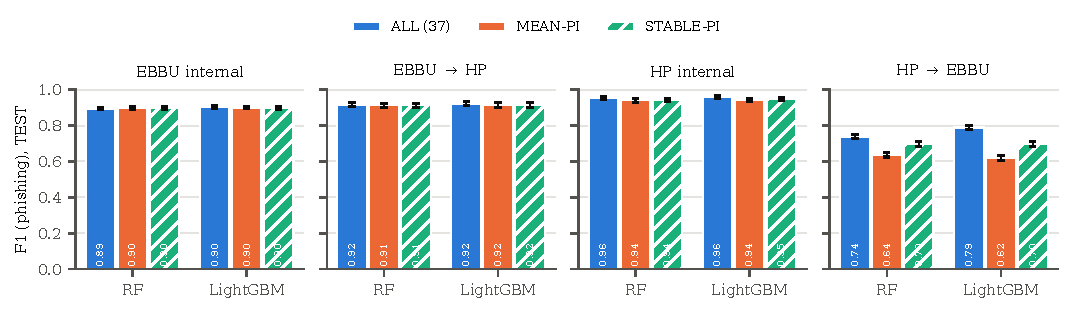
\includegraphics[width=\textwidth]{generated/fig_f1.pdf}
\caption{F1 on TEST for the four evaluation cells (bars: mean of 3 seeds; whiskers: 95\% domain-cluster bootstrap CI). Feature sets: ALL (blue), MEAN-PI (orange), STABLE-PI (green, hatched).}
\label{fig:f1}
\end{figure*}

\subsection{RQ2: stability-based versus mean-importance selection}
Table~\ref{tab:contrasts} lists the four pre-specified contrasts. In EBBU$\rightarrow$HP, differences between STABLE-PI and MEAN-PI are small (RF \res{DeltaABRF} [\res{DeltaLoABRF}, \res{DeltaHiABRF}], LightGBM \res{DeltaABLGBM} [\res{DeltaLoABLGBM}, \res{DeltaHiABLGBM}]) relative to the pre-set practical band. We do not claim statistical equivalence. In HP$\rightarrow$EBBU, the paired differences favour STABLE-PI: \res{DeltaBARF} [\res{DeltaLoBARF}, \res{DeltaHiBARF}] for RF and \res{DeltaBALGBM} [\res{DeltaLoBALGBM}, \res{DeltaHiBALGBM}] for LightGBM; the sign is positive in every seed, although the size varies (Table~\ref{tab:contrasts}). Internally, the observed selector differences are below the practical threshold.

The secondary contrasts temper this result: reduced subsets did not match ALL across both datasets. On HP$\rightarrow$EBBU, the STABLE-PI minus ALL F1 differences are \res{SecBARFSTABLEALL} (RF) and \res{SecBALGBMSTABLEALL} (LightGBM), while MEAN-PI minus ALL gives \res{SecBARFMEANALL} and \res{SecBALGBMMEANALL}. Stability ranking mitigates the loss associated with these compact configurations, without recovering ALL performance. This does not prove that the feature count alone causes the loss; membership and fitted trees also differ. On EBBU$\rightarrow$HP the STABLE-PI minus ALL differences are \res{SecABRFSTABLEALL} and \res{SecABLGBMSTABLEALL}.

\begin{table*}[t]
\caption{Paired domain-cluster bootstrap contrasts of target-TEST F1 (\res{nBoot} replicates; same resampled domains for both arms and all seeds). Top: the four primary contrasts; bottom: secondary cross-dataset contrasts. Per-seed deltas for seeds 17/29/43.}
\label{tab:contrasts}
\centering\scriptsize
\begin{tabular}{lllcccc}
\toprule
Cell & Model & Contrast & $k$ & $\Delta$F1 & 95\% CI & per seed \\
\midrule
A$\rightarrow$B & RF & STABLE vs MEAN (matched $k$) & 16/16/16 vs 16/16/16 & -0.000 & [-0.001, +0.000] & +0.000 +0.002 -0.004 \\
A$\rightarrow$B & LGBM & STABLE vs MEAN (matched $k$) & 16/16/16 vs 16/16/16 & -0.000 & [-0.001, +0.000] & +0.000 -0.002 +0.001 \\
B$\rightarrow$A & RF & STABLE vs MEAN (matched $k$) & 8/8/8 vs 8/8/8 & +0.059 & [+0.051, +0.066] & +0.095 +0.014 +0.066 \\
B$\rightarrow$A & LGBM & STABLE vs MEAN (matched $k$) & 8/8/8 vs 8/8/8 & +0.077 & [+0.069, +0.086] & +0.073 +0.039 +0.120 \\
\midrule
A$\rightarrow$B & RF & STABLE vs ALL & 16/16/16 vs 37/37/37 & -0.004 & [-0.006, -0.003] & -0.001 -0.002 -0.010 \\
A$\rightarrow$B & RF & MEAN vs ALL & 16/16/16 vs 37/37/37 & -0.004 & [-0.005, -0.002] & -0.001 -0.005 -0.006 \\
A$\rightarrow$B & RF & STABLE vs MEAN (budget $k$) & 16/16/16 vs 16/16/16 & -0.000 & [-0.001, +0.000] & +0.000 +0.002 -0.004 \\
A$\rightarrow$B & LGBM & STABLE vs ALL & 16/16/16 vs 37/37/37 & -0.007 & [-0.009, -0.004] & -0.007 -0.007 -0.006 \\
A$\rightarrow$B & LGBM & MEAN vs ALL & 16/16/16 vs 37/37/37 & -0.006 & [-0.009, -0.004] & -0.007 -0.005 -0.007 \\
A$\rightarrow$B & LGBM & STABLE vs MEAN (budget $k$) & 16/16/16 vs 16/16/16 & -0.000 & [-0.001, +0.000] & +0.000 -0.002 +0.001 \\
B$\rightarrow$A & RF & STABLE vs ALL & 8/8/8 vs 37/37/37 & -0.042 & [-0.050, -0.033] & -0.048 -0.027 -0.049 \\
B$\rightarrow$A & RF & MEAN vs ALL & 8/8/8 vs 37/37/37 & -0.100 & [-0.109, -0.092] & -0.143 -0.041 -0.116 \\
B$\rightarrow$A & RF & STABLE vs MEAN (budget $k$) & 8/8/8 vs 8/8/8 & +0.059 & [+0.051, +0.066] & +0.095 +0.014 +0.066 \\
B$\rightarrow$A & LGBM & STABLE vs ALL & 8/8/8 vs 37/37/37 & -0.093 & [-0.101, -0.085] & -0.093 -0.093 -0.093 \\
B$\rightarrow$A & LGBM & MEAN vs ALL & 8/8/8 vs 37/37/37 & -0.170 & [-0.181, -0.159] & -0.166 -0.132 -0.212 \\
B$\rightarrow$A & LGBM & STABLE vs MEAN (budget $k$) & 8/8/8 vs 8/8/8 & +0.077 & [+0.069, +0.086] & +0.073 +0.039 +0.120 \\
\bottomrule
\end{tabular}

\end{table*}

\subsection{RQ3: computational cost}
Table~\ref{tab:cost} and Fig.~\ref{fig:latency} give the latency per URL. For a single URL on one thread, reduced subsets take \res{relLatB1Min}--\res{relLatB1Max} of the end-to-end time of the corresponding ALL model; for batches of 1{,}024 URLs on four threads the ratio is \res{relLatBkMin}--\res{relLatBkMax}. Parsing and feature extraction account for a median of \res{extractShareMedian}\% of single-URL end-to-end time, so pruning features mainly saves extraction work, while tree inference cost depends little on the number of input features.

\begin{table*}[t]
\caption{Cost of the seed-17 model of every configuration (median $\mu$s per URL; ``rel.'' = end-to-end time relative to ALL of the same source and classifier). Hardware: \res{cpu}, \res{ram} GB RAM, Python \res{pyver}.}
\label{tab:cost}
\centering\scriptsize
\begin{tabular}{lllrrrrrrrrr}
\toprule
 & & & & \multicolumn{4}{c}{batch 1, 1 thread ($\mu$s/URL)} & \multicolumn{2}{c}{batch 1024, 4 thr.} & & \\
\cmidrule(lr){5-8}\cmidrule(lr){9-10}
Src & Model & Features & $k$ & extract & predict & e2e & rel. & e2e $\mu$s/URL & rel. & MB & fit s \\
\midrule
A & LGBM & MEAN-PI & 16 & 172 & 821 & 888 & 0.76 & 74.3 & 0.66 & 0.99 & 0.6 \\
A & LGBM & STABLE-PI & 16 & 177 & 598 & 881 & 0.75 & 75.0 & 0.67 & 0.99 & 0.6 \\
A & LGBM & ALL & 37 & 252 & 908 & 1167 & 1.00 & 112.5 & 1.00 & 1.00 & 0.8 \\
A & RF & MEAN-PI & 16 & 131 & 9881 & 9995 & 0.83 & 122.2 & 0.81 & 55.75 & 2.7 \\
A & RF & STABLE-PI & 16 & 112 & 9575 & 10110 & 0.84 & 121.0 & 0.81 & 55.75 & 2.7 \\
A & RF & ALL & 37 & 155 & 10244 & 12094 & 1.00 & 150.3 & 1.00 & 56.45 & 3.1 \\
B & LGBM & MEAN-PI & 8 & 150 & 539 & 772 & 0.93 & 61.0 & 0.55 & 0.99 & 0.6 \\
B & LGBM & STABLE-PI & 8 & 146 & 486 & 721 & 0.87 & 52.6 & 0.47 & 0.99 & 0.5 \\
B & LGBM & ALL & 37 & 228 & 556 & 830 & 1.00 & 111.3 & 1.00 & 1.00 & 0.9 \\
B & RF & MEAN-PI & 8 & 105 & 10316 & 10795 & 1.10 & 152.1 & 1.01 & 45.91 & 1.7 \\
B & RF & STABLE-PI & 8 & 111 & 10704 & 10455 & 1.06 & 92.7 & 0.61 & 44.15 & 1.5 \\
B & RF & ALL & 37 & 150 & 9356 & 9852 & 1.00 & 151.1 & 1.00 & 41.45 & 3.6 \\
\bottomrule
\end{tabular}

\end{table*}

\subsection{RQ4: attributions}
The corrected exploratory explanations pass strict additivity (maximum residual \res{shapAddErr}). The following rankings use these corrected outputs; the original failing outputs remain archived. Numerical consistency does not establish causal attribution or complete explanation fidelity.
SHAP rankings of the same model on source and target TEST samples agree to a Spearman $\rho$ of \res{rhoMin}--\res{rhoMax} (Table~\ref{tab:shap}, Fig.~\ref{fig:shap}); seed-to-seed agreement of the ALL models on the source is at least \res{rhoSeedMin}. Fig.~\ref{fig:pi} shows the permutation-importance evidence from which the subsets were drawn. Because the input distribution changes between cohorts, a different ranking on the target describes \emph{what} the model used there; it is not by itself evidence of an unfaithful explanation, nor of a causal role of a feature.

\begin{table*}[t]
\caption{Exploratory corrected SHAP rank agreement: source vs.\ target TEST ($\rho$, top-10 Jaccard) and across seeds for ALL; top-5 features on the source.}
\label{tab:shap}
\centering\scriptsize
\begin{tabular}{lllcccp{3.2cm}}
\toprule
Dir. & Model & Features & $\rho_{\mathrm{src,tgt}}$ & J$_{10}$ & $\rho_{\mathrm{seeds}}$ & top-5 (source) \\
\midrule
A$\rightarrow$B & LGBM & ALL (37) & 0.99 & 0.82 & 1.00 & \scriptsize F23 F09 F30 F06 F03 \\
A$\rightarrow$B & LGBM & STABLE-PI & 0.88 & 0.82 & -- & \scriptsize F23 F09 F03 F06 F30 \\
A$\rightarrow$B & RF & ALL (37) & 0.97 & 0.82 & 1.00 & \scriptsize F23 F09 F30 F07 F03 \\
A$\rightarrow$B & RF & STABLE-PI & 0.81 & 0.82 & -- & \scriptsize F23 F09 F03 F30 F07 \\
B$\rightarrow$A & LGBM & ALL (37) & 0.96 & 0.82 & 1.00 & \scriptsize F02 F23 F06 F03 F22 \\
B$\rightarrow$A & LGBM & STABLE-PI & 0.98 & 1.00 & -- & \scriptsize F02 F23 F03 F06 F21 \\
B$\rightarrow$A & RF & ALL (37) & 0.95 & 0.82 & 1.00 & \scriptsize F02 F23 F06 F01 F03 \\
B$\rightarrow$A & RF & STABLE-PI & 0.98 & 1.00 & -- & \scriptsize F02 F23 F06 F03 F21 \\
\bottomrule
\end{tabular}

\end{table*}

\begin{figure*}[t]
\centering
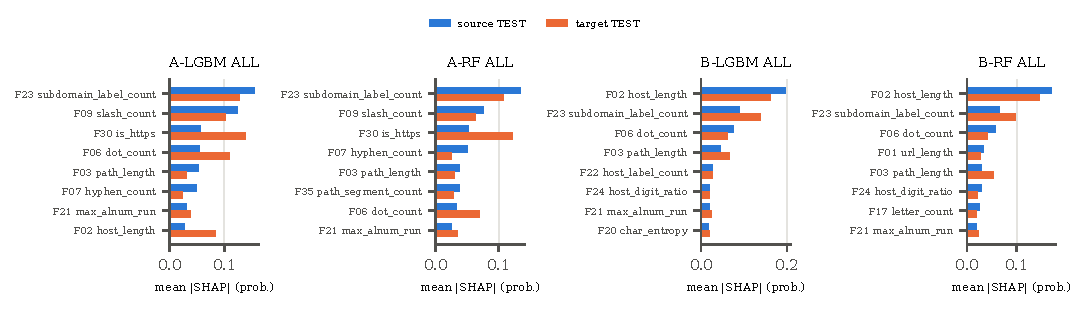
\includegraphics[width=\textwidth]{generated/fig_shap.pdf}
\caption{Exploratory corrected mean $|$SHAP$|$ (probability scale) of the eight most important features of the seed-17 ALL models on source TEST (blue) and target TEST (orange).}
\label{fig:shap}
\end{figure*}

\begin{figure*}[t]
\centering
\begin{minipage}[t]{0.48\textwidth}
\centering\vspace{0pt}
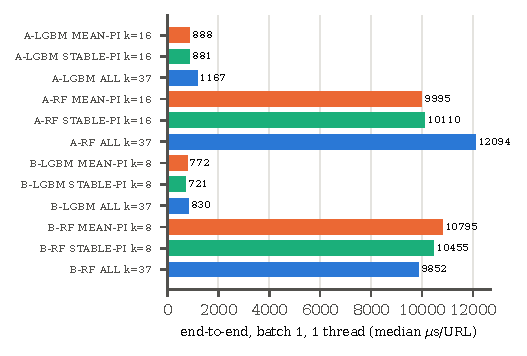
\includegraphics[width=\linewidth]{generated/fig_latency.pdf}
\caption{End-to-end latency for a single URL on one thread (seed-17 models).}
\label{fig:latency}
\end{minipage}\hfill
\begin{minipage}[t]{0.48\textwidth}
\centering\vspace{0pt}
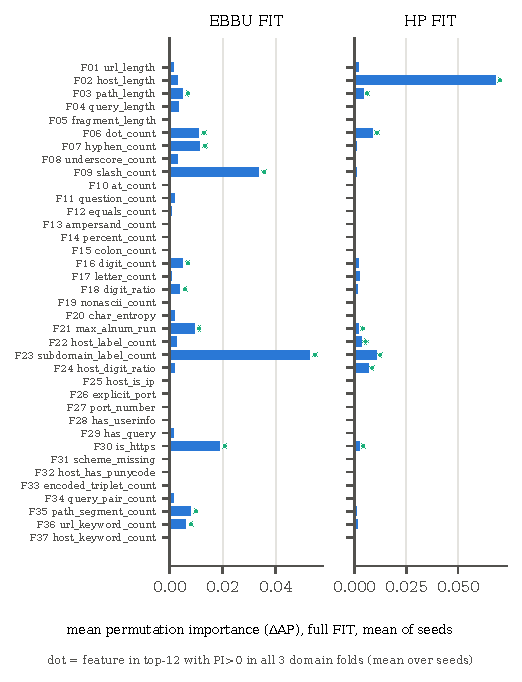
\includegraphics[width=\linewidth]{generated/fig_pi.pdf}
\caption{Permutation importance on full FIT (mean over folds and seeds). Dots mark features that are in the top 12 with positive PI in all three domain folds.}
\label{fig:pi}
\end{minipage}
\end{figure*}

\section{Discussion}
\textit{Interpreting transfer asymmetry.} The FIT partitions show descriptive source differences: HP benign URLs are short (median \res{medLenBBenign} characters) and mostly HTTPS (\res{httpsBBenign}\%), whereas HP phishing URLs are longer (\res{medLenBPhish}) with more dots and subdomains (medians \res{medDotsBPhish} and \res{medSubBPhish}). In EBBU, phishing URLs have medians of \res{medSubAPhish} subdomains and \res{medDotsAPhish} dots and are rarely HTTPS (\res{httpsAPhish}\%), but neither are its benign URLs (\res{httpsABenign}\% HTTPS). The RQ5 diagnostics turn this description into a mechanism. Some cues are shared in direction (HTTPS, length, entropy), others reverse (host-label and subdomain counts, query presence). EBBU-trained models meet HP data in which the main errors are HTTPS phishing, a population that barely exists in EBBU. HP-trained models meet EBBU data whose benign URLs lack the \texttt{www} label and whose phishing URLs carry few subdomains, contrary to what HP taught them. The slice error rates are consistent with this account; they remain correlational and do not prove that a single feature caused an individual error. Rashid~\textit{et al.}~\cite{rashid2024} already discuss feature-distribution differences, so identifying source shift is not our novelty. The two datasets differ in collection process, period and prevalence; our transfer drop describes this benchmark pair rather than isolating a causal domain-shift effect.

\textit{What does stability buy?} STABLE-PI prioritises features with more positive top-$q$ fold votes; it does not require every selected feature to be stable in all folds and does not guarantee invariance across datasets. It outperformed mean ranking at the same small budget in HP$\rightarrow$EBBU, without a clear advantage in the other direction. The matched-$k$ design separates this ranking comparison from the number of retained features. ALL nevertheless remained the stronger cross-dataset reference. Our empirical insight is therefore conditional: source-domain stability can mitigate the loss from a compact subset in this benchmark, but it does not establish that source-selected compression preserves transfer or that the rule is generally safer. RQ5 shows why. Stability is measured across folds of \emph{one} collection, so it rewards features that are consistently useful there, including features whose class association reverses elsewhere. ALL keeps more redundant cues and so has more ways to recover when one cue fails. Stability across \emph{sources}, rather than across folds, is what would be needed, and that requires a second labelled source (Section~\ref{sec:future}).

\textit{What the two-paper extension establishes.} We connect the classifier/representativeness questions in~\cite{sanchez2022} with the transfer problem in~\cite{rashid2024} through a controlled source-only evaluation. Both primary papers satisfy the five-year recency limit; original EBBU provenance is retained in the repository. The contribution lies in the auditable protocol and the ranking--budget--cost comparison. We have not run either original system under identical conditions, so we cannot attribute improvements over their published results to our approach. The two primary papers satisfy the revised project count and recency conditions; they do not establish universal novelty, and relevant adjacent work remains acknowledged.

\textit{Did we get what we wanted?} Partly. The hypothesis that stability-based selection transfers better than mean importance at equal budgets was supported in one direction and neutral in the other. The broader hope that a compact, cheaper model could keep cross-dataset accuracy was not supported: no subset matched ALL, and the latency gains are modest. The study did deliver a clear negative result and a mechanism, which matters for practice: a lexical detector that looks strong on one collection can depend on period-specific cues such as HTTPS.

\textit{What we would do differently.} We would (i) include LogReg and the one-feature rule as pre-registered baselines rather than post-freeze diagnostics; (ii) plan class-conditional feature analysis of both sources \emph{before} defining the selectors, which would have motivated a cross-source criterion; (iii) budget for a third source from the start, so that selection evidence and evaluation come from different collections; and (iv) separate threshold transfer from ranking transfer in the primary outcome, by reporting AP-based contrasts next to F1.

\textit{Uncertainty.} The bootstrap intervals resample target domains for fixed fitted models; they do not include resampling or split-induced training variability. Table~\ref{tab:contrasts} shows that per-seed differences vary, so the size of the advantage is less stable than its observed sign. Three estimator seeds on a single split do not establish a population-level training effect, and we make no family-wise significance claim. Additional independently collected holdout data and repeated training splits would strengthen robustness claims, but must be planned under a new protocol before opening a new holdout.

\textit{Cost.} Lexical models are already cheap; reducing 37 to 8--16 features trims extraction work but the shared parsing step and the per-call overhead of the model remain, so savings are modest relative to the accuracy given up on the hard direction. ``Lightweight'' is therefore relative to the ALL model on the reported hardware.

\textit{Threats to validity.} (i) Both datasets are older public collections; results do not establish contemporary or zero-day robustness. (ii) The symmetric purge removes shared popular domains and changes the evaluation population. (iii) Both selectors share an RF proxy, which may favour RF. (iv) Correlated lexical features can depress PI. (v) Hyper-parameters were fixed, not optimised. (vi) HP encoding is crossvalidated against the primary paper's class counts in all original splits; a verbatim numeric codebook is not supplied. The complete user-supplied article PDF was reviewed, including its data, alignment algorithm and limitations. (vii) RQ5 is exploratory, post-freeze and computed on VAL of a single split; source-VAL F1 is optimistic because it also sets thresholds. (viii) The freeze is a procedural control, signed by an agent on the author's instruction. (ix) The original SHAP outputs failed additivity and the legacy analysis accessed TEST labels outside the evaluator. Both findings remain in the v1 audit trail. This version uses a separately hashed, label-free exploratory correction on saved feature matrices, with strict additivity and classifier-equivalence checks. Correction after observing v1 outputs does not create a new independent holdout or establish causal explanation fidelity. Full-text review of the primary papers supports this methodological distinction without establishing global novelty.

\section{Future Work}\label{sec:future}
Four directions follow directly from the findings. \emph{(i) A third source.} DA-GAFS selects with two labelled collections and is evaluated on held-out domains of the same collections; a confirmatory test must select on two sources and evaluate on a third, untouched one, under a new protocol version and holdout. \emph{(ii) Conditional direction.} The marginal direction gate removed a reversed but useful cue; replacing it with a conditional criterion, such as sign agreement of SHAP attributions within comparable slices, or penalising rather than excluding conflicts, is the natural refinement of C2. \emph{(iii) Contemporary and temporal data.} Both datasets are older public collections in which HTTPS is a strong benign cue; repeating the protocol on recent feeds with a temporal split would test whether this cue still transfers. \emph{(iv) Threshold transfer.} Ranking can partly transfer while the source threshold does not; label-free recalibration from target score distributions, compared with UDA~\cite{rashid2024} under the same domain-disjoint splits, would separate representation shift from operating-point shift. None of these may reuse the present TEST data for model choice.

\section{Conclusion}
On a domain-disjoint EBBU/HP benchmark with a frozen, source-only learning protocol, lexical URL classifiers transferred well from EBBU to HP (F1 \res{F1ABLGBMALL} for LightGBM) but lost \res{DropBLGBMALL}--\res{DropBRFALL} F1 points from HP to EBBU (RQ1). Stability ranking gave higher target F1 than mean ranking at the same budget in the harder direction (\res{DeltaBARF} RF, \res{DeltaBALGBM} LightGBM), without a clear advantage in the other direction; reduced subsets did not match the full feature set across datasets (RQ2). Latency trade-offs depend on the model and execution setting (RQ3). Exploratory corrected SHAP comparisons pass strict numerical additivity while retaining descriptive, non-causal scope (RQ4). Exploratory baselines and error analysis on validation data (RQ5) show why: tree ensembles transfer far better than logistic regression, an HTTPS-only rule already explains much of the easy direction, and features whose class association reverses between collections cannot be identified by any source-only selector. The contribution is a reproducible empirical comparison under a defined target-access constraint, not a new classifier or a demonstrated improvement over UDA. Section~\ref{sec:future} outlines the next experiments.

\section*{Data and Code Availability}
Raw data are not redistributed (licences unclear); the package downloads EBBU (\url{https://github.com/ebubekirbbr/pdd}, commit \texttt{90b394d}) and HP (\url{https://github.com/fariza25/PhishingURLDetection}, commit \texttt{ff9f1f5}) at pinned commits and verifies SHA256 hashes. Code, notebook and slides: \url{https://github.com/Athraynmhd/phishing-url-generalization}. Code, configuration, lockfile, schemas, decision log and the freeze manifest (\texttt{\res{freezeHash}}) are in the project repository; every empirical number in this paper is read from this bundle's automatically generated \texttt{generated/macros.tex}. Correction provenance links its SHAP inputs to the preserved v1 outputs.


\bibliographystyle{IEEEtran}
\bibliography{refs}

\end{document}
